\documentclass[journal]{IEEEtran}

% IEEE Transactions on Vehicular Technology uses the standard IEEEtran journal
% format. This draft is organized for a TVT-style communication/perception paper.

\usepackage{amsmath,amssymb}
\usepackage{graphicx}
\usepackage{booktabs}
\usepackage{multirow}
\usepackage{cite}
\usepackage{xcolor}
\usepackage{url}

\graphicspath{{figures/}}

\newcommand{\todo}[1]{\textcolor{red}{[TODO: #1]}}
\newcommand{\method}{CA-TOSG}

\begin{document}

\title{Channel-Aware Task-Oriented Semantic Granularity Selection for Bandwidth-Constrained V2V Cooperative Perception}

\author{
Peiyi Yue%
\thanks{Peiyi Yue is with the Department of Electrical and Electronic Engineering, University of Bristol, Bristol, UK (e-mail: pyyue9836@gmail.com).}
}

\markboth{IEEE Transactions on Vehicular Technology,~Vol.~XX, No.~X, 2026}
{Yue: Channel-Aware Semantic Granularity Selection for V2V Cooperative Perception}

\maketitle

\begin{abstract}
Connected and automated vehicles can improve perception reliability by exchanging information through vehicle-to-vehicle (V2V) links. However, cooperative perception must operate under limited bandwidth and time-varying vehicular channels. Existing communication-efficient perception methods mainly reduce redundancy within a fixed semantic representation, such as object-level detections or feature-level messages. This paper shows that fixed semantic granularity is suboptimal: feature-level messages are potentially more informative but can become unreliable or wasteful under poor channel quality, while object-level messages are compact and stable but less expressive. We propose \emph{Channel-Aware Task-Oriented Semantic Granularity Selection} (\method), a receiver-driven framework in which the ego vehicle selects the communication granularity for each frame from its own perception cues and estimated channel state, and signals the choice to the collaborator via a $2$-bit request piggy-backed on periodic V2X awareness messages, such as CAM/BSM, over 802.11bd or NR sidelink. \method{} chooses one message type from object-level communication and compressed feature-level communication modes before any high-payload transmission. We derive the selector as the Lagrangian-relaxed solution of a constrained perception-communication problem and instantiate it with a $400$-tree Random Forest. Experiments on the OPV2V dataset (validate, scene-disjoint test, and the Culver-City domain shift) under AWGN and Rayleigh channels show that, when the channel can carry feature-level messages, \method{} lifts true end-to-end AP@0.5 by up to $+0.07$ over object-level communication where the channel carries feature-level messages (Culver-City), remaining comparable to object-level on the easier test split, while---averaged over all channel states---using $16$--$25\%$ of the per-frame channel use of fixed $C_{16}$ feature-level transmission under rate-1/2 LDPC + 16-QAM coding; under fading it safely falls back to the robust object-level message. The estimated SNR and channel-type features jointly account for $62\%$ of the selector's feature importance, dominating $21$ ego-side cues. Crucially, the feature codec's channel response determines the \emph{currency} in which the perception cues pay: under an LDPC + QAM cliff the estimated SNR is a near-sufficient statistic---cues add no significant realised-F1 gain over channel state alone yet cut channel use by ${\approx}12\%$ at matched F1---whereas under graceful importance-map JSCC the SNR becomes uninformative and the cue-based selector beats the best SNR threshold by $+0.027$ realised F1 ($95\%$ CI $[+0.024,+0.029]$); under deep fading the codec instead sets feasibility, the digital feature branch turning infeasible over the evaluated SNR range while analog JSCC survives. The deployed selector incurs $52.8$~ms per frame on a single CPU core, fitting the $100$~ms budget of a 10~Hz LiDAR cycle. These results demonstrate that channel-aware semantic granularity adaptation is an effective strategy for bandwidth-constrained V2V cooperative perception.
\end{abstract}

\begin{IEEEkeywords}
Vehicle-to-vehicle communication, cooperative perception, connected vehicles, semantic communication, 3D object detection, channel-aware communication.
\end{IEEEkeywords}

\section{Introduction}

Connected and automated vehicles are expected to rely not only on their onboard sensors, but also on information shared by surrounding vehicles. By exchanging perception information through vehicle-to-vehicle (V2V) links, a vehicle can obtain complementary viewpoints and improve its understanding of the driving scene. This capability is particularly important in safety-critical scenarios such as intersections, dense traffic, occluded road segments, and long-range perception, where a single vehicle's LiDAR or camera may provide incomplete observations. Cooperative perception therefore has the potential to improve detection robustness beyond the physical sensing range and viewpoint of an individual vehicle~\cite{xu2022opv2v,xu2022v2xvit}.

Despite this potential, practical V2V cooperative perception is fundamentally constrained by communication. Sharing raw point clouds or dense intermediate feature maps can preserve rich geometric and semantic information, but the resulting payload can be too large for vehicular links with limited bandwidth and latency requirements. Moreover, V2V channels are time-varying due to mobility, blockage, multipath propagation, and fading~\cite{ieee80211bd,3gpp38885}. A communication strategy that is effective under a clean channel may become unreliable under low signal-to-noise ratio (SNR) or fading. Therefore, cooperative perception cannot be designed only as a perception problem; it must also account for the reliability and cost of the vehicular communication link.

Existing cooperative perception methods make different choices along the perception-communication trade-off. Late-fusion methods transmit object-level predictions, such as 3D bounding boxes, class labels, and confidence scores~\cite{xu2022opv2v}. These messages are compact and can be protected with strong coding, but they discard intermediate semantic context and may suffer when local detections are uncertain or incomplete. Intermediate-fusion methods transmit learned feature maps, which usually provide richer information for downstream fusion and detection~\cite{xu2022v2xvit,hu2022where2comm}, but at a much higher communication cost. Recent communication-efficient methods reduce this cost by selecting important feature regions, applying attention-based masks, or compressing feature representations~\cite{hu2022where2comm}. Semantic communication and joint source-channel coding methods further optimize the transmitted feature representation for task performance under wireless channels~\cite{sheng2024importance,gan2026scomcp}.

However, most existing methods operate within a fixed semantic granularity. Object-level approaches always transmit object-level messages, while feature-level approaches always transmit feature-level messages, even if only a subset of feature tokens is selected. Thus, many methods answer the question of \emph{which feature elements should be transmitted}, but do not explicitly answer a higher-level question: \emph{whether feature-level communication is needed for the current frame at all}. This distinction is important in vehicular systems. In some frames, local perception may already be confident and stable, making compact object-level communication sufficient. In other frames, such as those with occlusion or ambiguous detections, richer feature-level communication may provide useful information for fusion. The best communication granularity is therefore not fixed, but depends on the task state of the perception system.

The communication channel further changes this decision. Feature-level messages are potentially more informative, but they are also more sensitive to channel degradation because larger and denser messages require more reliable transmission. Under poor SNR or fading, a feature-level message may be corrupted or effectively unusable, making its additional payload wasteful or even harmful for task performance. In contrast, object-level messages are much smaller and can be treated as robust low-rate information in many system designs. As a result, richer semantic communication does not always lead to better cooperative perception. The optimal message granularity depends jointly on perception task cues and channel quality.

Motivated by this observation, this paper proposes \emph{Channel-Aware Task-Oriented Semantic Granularity Selection} (\method) for bandwidth-constrained V2V cooperative perception. Instead of transmitting a fixed representation for every frame, \method{} selects one message type from a set of semantic communication candidates. In the considered implementation, the selector chooses among an object-level message and compressed feature-level messages with different channel-use characteristics. The decision is made using ego-side task cues, such as prediction confidence, visibility, temporal stability, and detection uncertainty, together with estimated channel quality such as SNR. The selected message is then transmitted through the V2V link and fused with the ego vehicle's local feature for 3D object detection. An overview of the resulting framework is shown in Fig.~\ref{fig:overview}.

\begin{figure*}[t]
    \centering
    
\includegraphics[width=\textwidth]{ca_tosg_method_overview.pdf}
    \caption{Overview of the proposed \method{} framework. The sender extracts online task cues $z_t$ and estimated channel quality $(\gamma_t,\text{ch}_t)$, then selects one communication mode $s_t \in \{L,C_{16},C_{256}\}$. Only the selected message is transmitted through the V2V link and fused with the local ego feature $F_{\mathrm{ego},t}$ for 3D object detection.}
    \label{fig:overview}
\end{figure*}

This formulation is complementary to existing feature compression and semantic communication methods. A feature codec, sparse feature selector~\cite{hu2022where2comm}, or joint source-channel coding module~\cite{sheng2024importance,gan2026scomcp} can be used inside the feature-level branch. \method{} operates one level above these modules by deciding when feature-level communication should be activated. This is especially relevant for vehicular networks, where unnecessary high-payload communication should be avoided when the channel cannot support reliable feature transmission or when the current frame does not require additional semantic detail.

The main contributions of this paper are summarized as follows:
\begin{itemize}
    \item We formulate channel-aware semantic granularity selection for V2V cooperative perception, where the sender adaptively selects the semantic level of each transmitted message according to task state and channel quality.
    \item We instantiate the framework as a lightweight, interpretable, receiver-driven policy that uses only ego-side perception cues and an estimated SNR/channel-type, adds no learnable parameters to the perception backbone, and runs in real time on a single CPU core. The policy is deliberately model-agnostic: a $400$-tree Random Forest~\cite{breiman2001random} and a one-line SNR threshold are two interchangeable realisations, so the contribution is the \emph{selection framework}, not a particular classifier.
    \item We provide a communication-aware evaluation protocol under AWGN and Rayleigh channels, comparing fixed object-level transmission, fixed feature-level transmission with LDPC + 16/256-QAM coding~\cite{ieee80211bd}, a learned semantic-communication baseline~\cite{sheng2024importance}, and a channel-aware oracle.
    \item Experiments on OPV2V show that \method{} avoids unreliable high-payload feature transmission under poor channel conditions and approaches oracle performance when the channel supports richer communication. We characterise it as \emph{Pareto-optimal} on the payload--F1 plane rather than merely better on average, show the gain concentrates on the hardest frames under a usable channel (up to $+0.11$ F1 on the low-tercile frames, AWGN $16$~dB), and verify cross-split and Culver-City domain-shift generalisation with a frozen selector.
    \item Our central finding is that the feature codec's channel response \emph{determines the currency in which the task cues pay}: under an LDPC + QAM cliff the estimated SNR is a near-sufficient statistic---perception cues add no significant realised-F1 gain over channel state alone yet cut the selector's channel use by ${\approx}12\%$ at matched F1---whereas under graceful importance-map JSCC the SNR becomes uninformative, the best SNR threshold collapses to object-level performance, and the cue-based selector beats it by $+0.027$ realised F1 ($95\%$ CI $[+0.024,+0.029]$, AWGN test; $+0.022$ under Rayleigh and $+0.025$ under OFDM). Under deep fading the codec choice instead sets \emph{feasibility}: the digital LDPC feature branch is infeasible over the evaluated SNR range, its frame-error threshold rising as the diversity order falls---$8$~dB on AWGN, ${\sim}24$~dB under OFDM (empirical diversity order ${\approx}2$), and unbounded under flat Rayleigh---while analog JSCC survives the fading and keeps the selector valuable. This identifies precisely when a task-oriented selector is necessary versus when channel state alone suffices.
\end{itemize}

\section{Related Work}

\subsection{V2V Cooperative Perception}

V2V cooperative perception aims to improve the perception capability of an ego vehicle by exploiting information from surrounding connected vehicles~\cite{xu2022opv2v,han2023collaborative}. Compared with single-agent perception, cooperative perception can provide complementary viewpoints and alleviate occlusion, long-range sparsity, and limited field-of-view problems. Existing methods are commonly categorized according to the stage at which information is shared: early fusion, intermediate fusion, and late fusion.

Early fusion shares raw sensor measurements, such as point clouds, among vehicles before feature extraction~\cite{xu2022opv2v}. Since raw observations preserve the most complete information, early fusion can potentially provide strong perception performance. However, it introduces a very large communication payload and requires accurate spatial and temporal alignment across agents. These limitations make raw-data sharing difficult to deploy under practical V2V bandwidth and latency constraints.

Late fusion shares compact object-level predictions, including 3D bounding boxes, class labels, and confidence scores~\cite{xu2022opv2v}. This strategy has a much smaller payload and is naturally compatible with low-rate V2V communication. However, late fusion discards intermediate semantic and spatial information. Once an object is missed or incorrectly detected by the sender, the receiver has limited ability to recover from the error. As a result, late fusion is efficient but may be less effective in challenging scenes with occlusion or uncertain local detections.

Intermediate fusion shares learned feature representations, such as BEV feature maps, after local backbone extraction and before the final detection head~\cite{xu2022v2xvit,hu2022where2comm,wang2020v2vnet,li2021disconet,xu2022cobevt,liu2020when2com,lu2024heal,hu2024pragmatic}. Many cooperative perception frameworks adopt intermediate fusion because it offers a favorable balance between raw-data sharing and object-level sharing. By exchanging intermediate features, the ego vehicle can fuse richer spatial and semantic information from neighboring vehicles. However, intermediate features are still much larger than object-level messages, and their transmission can be expensive under bandwidth-constrained V2V links.

Recent benchmarks and toolkits, such as OPV2V and OpenCOOD~\cite{xu2022opv2v}, have enabled systematic evaluation of cooperative perception methods under realistic multi-agent driving scenarios. These platforms provide common datasets, model architectures, and evaluation protocols for comparing fusion strategies. In this paper, we build on this cooperative perception setting but focus on a different problem: rather than assuming a fixed fusion representation, we study how to select the semantic granularity of the transmitted message according to task and channel conditions.

\subsection{Communication-Efficient Cooperative Perception}

To reduce the communication burden of intermediate fusion, many methods aim to transmit only task-relevant features. A common strategy is to use confidence maps, attention weights, or importance masks to select informative spatial regions from the feature map~\cite{hu2022where2comm,sheng2024importance}. For example, spatially selective methods transmit only a subset of BEV tokens that are expected to contribute to downstream detection. This reduces redundant communication while retaining much of the benefit of feature-level cooperation.

Where2comm~\cite{hu2022where2comm} is a representative method in this direction. It estimates where communication is needed and selectively transmits spatial feature regions for cooperative perception. Such methods are effective because not all BEV locations contribute equally to object detection. Attention-based and confidence-based approaches follow a similar principle: they suppress unimportant feature regions and allocate communication resources to more informative areas.

Feature compression is another important direction. Instead of directly transmitting dense feature maps, the sender can encode them into a lower-dimensional representation before communication~\cite{sheng2024importance}. The receiver then decodes or fuses the compressed feature representation for detection. These approaches can reduce payload and may be combined with channel coding or learned semantic communication modules.

However, most communication-efficient cooperative perception methods still operate within a fixed semantic level. They usually assume that the system will transmit feature-level information and then optimize which feature tokens or compressed representations should be sent. A notable exception is ML-Cooper~\cite{xie2022mlcooper}, which employs a soft actor--critic reinforcement-learning policy to adapt the proportion of raw-, feature-, and object-level data shared according to the vehicular network state; this is the closest prior work to a channel-conditioned choice of message granularity, but its adaptation relies on a heavyweight learned policy and it does not characterize \emph{when} such granularity adaptation is genuinely required. In contrast, our work studies a higher-level yet lightweight and interpretable decision: whether the current frame should use feature-level communication at all. The proposed \method{} framework can select compact object-level communication when feature-level information is unnecessary or unreliable, and activate feature-level communication only when its expected task benefit justifies the additional payload. The granularity selection of \method{} is therefore orthogonal to the spatial selection of Where2comm or the codec design of importance-map JSCC~\cite{sheng2024importance}, and differs from ML-Cooper~\cite{xie2022mlcooper} in being a per-frame, interpretable selector rather than a reinforcement-learning policy; either compression module can be used inside the feature-level branch of our framework.

\subsection{Semantic and Channel-Aware Communication for Vehicular Perception}

Semantic communication has recently attracted attention as a task-oriented alternative to conventional bit-level communication~\cite{sheng2024importance,gan2026scomcp,bourtsoulatze2019deepjscc,xie2021deepsc,gunduz2023beyond}. Instead of minimizing reconstruction error or bit error rate alone, semantic communication optimizes the transmitted representation for downstream task performance. In cooperative perception, this means that the communication module should preserve information useful for detection, rather than reconstructing the full feature map perfectly.

Joint source-channel coding and learned semantic codecs provide one way to improve robustness under noisy wireless channels~\cite{sheng2024importance,gan2026scomcp}. By training the encoder and decoder with channel effects in the loop, these methods can produce representations that degrade more gracefully than conventional separated source and channel coding under certain channel conditions. Digital communication baselines, such as modulation and coding schemes based on QAM and LDPC, often show threshold or waterfall behavior~\cite{ieee80211bd}: performance can be poor below a certain SNR and improve rapidly once the channel becomes reliable.

For vehicular perception, this channel dependence is especially important. V2V links experience time-varying SNR, multipath propagation, blockage, and fading~\cite{ieee80211bd}. A feature-level message that is useful under a clean channel may become unreliable under low SNR or Rayleigh fading. Therefore, the semantic value of a transmitted message depends not only on its content but also on whether the channel can support its reliable delivery.

Existing semantic communication methods mainly focus on how to encode and transmit feature-level information more robustly. Some further make this transmission channel-adaptive at a fixed granularity: SmartCooper~\cite{zhang2024smartcooper} adjusts the feature compression ratio from the estimated channel state, while AccBEV~\cite{accbev2025} conditions a feature-repair module on the SNR to compensate for feature loss over lossy V2V links. These methods adapt \emph{how} the feature-level message is encoded or repaired, but still commit to feature-level transmission. Our work is complementary to these methods. A semantic codec or channel coding module can be used inside the feature-level branch of \method{}. The key difference is that \method{} operates before the transmission mode is chosen: it decides whether the sender should transmit object-level information or feature-level information under the current task and channel state. This channel-aware semantic granularity selection is particularly suitable for vehicular systems, where communication resources are limited and channel quality can change rapidly.

\section{System Model and Problem Formulation}\label{sec:system}

\subsection{Cooperative Perception Setting}

We consider a single ego--collaborator V2V link. At each frame $t$, the ego vehicle observes the scene using its onboard sensors and extracts a local bird's-eye-view (BEV) feature representation, denoted by $F_{\mathrm{ego},t}$. The collaborating vehicle also observes the scene from its own viewpoint and extracts a local feature representation $F_{j,t}$ using a shared PointPillars backbone~\cite{lang2019pointpillars}. The collaborator can transmit a perception message to the ego vehicle through the V2V link. The ego vehicle then fuses the received message with its local feature and produces the final 3D object detection output.

We adopt a \emph{receiver-driven} signalling architecture: the ego vehicle evaluates its own perception state and channel state, decides which semantic granularity is needed, and signals the choice to the collaborator using a $2$-bit request piggy-backed on the existing Cooperative Awareness Message (CAM) defined in IEEE~802.11bd~\cite{ieee80211bd}. The request thus costs $2$ bits per frame at $10$~Hz, i.e., $20$~bps, which is negligible relative to the $24$~kbit/s $L$ payload and is already provisioned in the standard CAM signalling budget. The collaborator complies by transmitting the requested message $m_t^{s_t}$. This receiver-driven design makes all perception cues used by the selector locally observable at the ego (Section~\ref{sec:cues}) and avoids any causality issues that would arise if the collaborator had to estimate ego-side perception state without feedback.

Let $Y_t$ denote the ground-truth objects at frame $t$, and let $\hat{Y}_t$ denote the predicted detection output at the ego vehicle after fusion. The objective of cooperative perception is to improve the task utility of $\hat{Y}_t$, such as average precision (AP) or F1 score, while keeping the V2V communication payload low. Unlike conventional cooperative perception settings that assume a fixed type of transmitted representation, we consider an ego-side selector that can choose the semantic granularity of the requested message according to both perception-side task cues and the estimated channel condition.

\subsection{Message Candidates}

At each frame, the sender selects one communication mode from a finite set of message candidates:
\begin{equation}
s_t \in \mathcal{S} = \{L, C_{16}, C_{256}\},
\label{eq:action_set}
\end{equation}
where $L$ denotes object-level communication, and $C_{16}$ and $C_{256}$ denote compressed feature-level communication modes associated with 16-QAM and 256-QAM modulation under rate-$1/2$ LDPC coding. The transmitted message is therefore
\begin{equation}
m_t = m_t^{s_t},
\end{equation}
where only the message corresponding to the selected mode $s_t$ is transmitted. This one-of-many design is important: the sender does not transmit both object-level and feature-level messages simultaneously, but chooses the semantic granularity that is expected to provide the best task-communication trade-off for the current frame.

The object-level message is defined as a compact set of local detections:
\begin{equation}
m_t^L = \{(b_k, c_k, p_k)\}_{k=1}^{N_t},
\end{equation}
where $N_t$ is the number of detected objects at the sender, $b_k$ is the 3D bounding box, $c_k$ is the class label, and $p_k$ is the confidence score of object $k$.

The compressed feature-level message is defined as
\begin{equation}
m_t^{C_q} = \phi_q(F_{j,t}), \quad q \in \{16, 256\},
\end{equation}
where $\phi_q(\cdot)$ denotes a feature encoding and communication process for mode $C_q$. The two feature-level modes carry the same perception payload of approximately $1.98$~Mbit but require different numbers of channel uses because of the different spectral efficiency of 16-QAM versus 256-QAM.

\subsection{Channel Model}

We consider a V2V link whose quality varies across frames. Let $\gamma_t$ denote the estimated channel quality at frame $t$, represented by the SNR in dB. The channel quality may be obtained from pilot-based estimation, link-layer feedback, or reference-signal-received-power reports as already produced by IEEE 802.11bd and 5G NR sidelink stacks~\cite{ieee80211bd}. In this work, we use $\gamma_t$ as an explicit input to the semantic granularity selector in order to study how channel awareness affects cooperative perception.

Two representative channel models are considered. The first is the additive white Gaussian noise (AWGN) channel, which models noise-limited transmission and provides a controlled setting for studying SNR-dependent behavior. The second is the Rayleigh fading channel, which captures multipath fading. The feature-level message under mode $C_q$ traverses the channel as a coded LDPC block, with block-error rate (BLER) function $\mathrm{BLER}_q(\gamma)$ that is monotonically non-increasing in $\gamma$ and exhibits the threshold behavior characteristic of LDPC decoding. We treat the object-level message $L$ as a low-rate robust message in the evaluated SNR range, motivated by its small payload (approximately $0.024$~Mbit) that allows aggressive channel coding or repeated transmission. Fig.~\ref{fig:bler} plots the resulting $\mathrm{BLER}_q(\gamma)$ for the LDPC + 16/256-QAM configurations under both channels, making explicit the threshold (cliff) behaviour that the selector must track.

\begin{figure}[t]
    \centering
    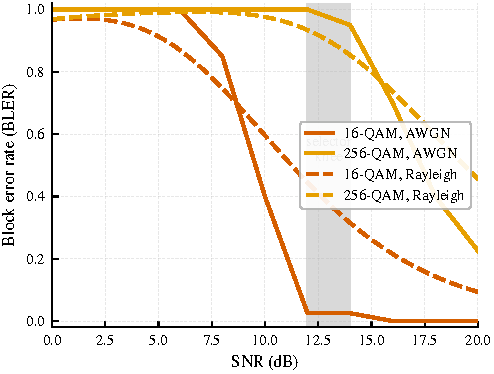
\includegraphics[width=\linewidth]{fig_channel_bler.pdf}
    \caption{Block-error rate of the feature-level message under LDPC $1/2$ with 16-QAM and 256-QAM, over AWGN (solid) and Rayleigh (dashed) channels. The 16-QAM AWGN cliff at $\approx 12$~dB defines the selector knee (shaded); the 256-QAM cliff sits far to its right, so by the time 256-QAM is reliable the 16-QAM block is already error-free---hence 256-QAM is dominated by 16-QAM under LDPC $1/2$. Under Rayleigh fading both curves degrade so slowly that feature-level transmission never becomes reliable in $0$--$20$~dB, explaining the selector's conservative $L$-only behaviour.}
    \label{fig:bler}
\end{figure}

\subsection{Effective Task Utility under Channel Corruption}

Let $F_t^s$ denote the realized frame F1 of the ego vehicle's detection output when the sender selects mode $s$ at frame $t$. We model the effective frame F1 under channel corruption as
\begin{align}
F_t^L      &= F_t^{L,\mathrm{clean}}, \label{eq:eff_L} \\
F_t^{C_q}  &= (1 - \mathrm{BLER}_q(\gamma_t,\text{ch}_t)) \cdot F_t^{C_q,\mathrm{clean}}, \quad q \in \{16, 256\}, \label{eq:eff_C}
\end{align}
where $\text{ch}_t \in \{\text{AWGN},\text{Rayleigh}\}$ and $F_t^{\cdot,\mathrm{clean}}$ denotes the frame F1 under perfect channel. Equation~\eqref{eq:eff_C} corresponds to a block-loss model: with probability $\mathrm{BLER}_q$ the feature-level message is unusable, contributing no detection benefit beyond the ego vehicle's own perception; with probability $1-\mathrm{BLER}_q$ it is delivered intact and contributes its clean F1. This is a conservative model; empirically, when a block is lost the receiver can fall back to ego-only inference rather than to a zero-utility state.

\subsection{Communication Cost}

Let $B_s$ denote the per-frame payload in channel-use-equivalent megabits for mode $s$, accounting for the spectral efficiency of the modulation:
\begin{equation}
B_L = 0.024, \quad B_{C_{16}} = 3.96/4 \approx 0.99, \quad B_{C_{256}} = 3.96/8 \approx 0.495,
\label{eq:payload}
\end{equation}
all in Mbit/frame, where $3.96 = 1.98/(1/2)$ is the coded-bit count produced by rate-$1/2$ LDPC from the $1.98$-Mbit feature payload, and the divisors $4$ and $8$ are the bits-per-symbol of 16-QAM and 256-QAM, respectively. The average communication cost over $T$ evaluated frames is
\begin{equation}
\bar{B} = \frac{1}{T}\sum_{t=1}^{T} B_{s_t} = \sum_{s \in \mathcal{S}} \rho_s B_s,
\end{equation}
where $\rho_s$ is the fraction of frames assigned to mode $s$. This equation highlights the role of semantic granularity selection: reducing the frequency of high-payload feature-level transmission directly reduces the average communication cost.

\subsection{Task-Communication Objective}

The goal of channel-aware semantic granularity selection is to choose a policy that balances detection utility and communication cost. Let $z_t$ denote the online task cue vector extracted from the ego-side perception stream, and let $\gamma_t$ denote the estimated channel quality. The selector is defined as
\begin{equation}
s_t = g(z_t, \gamma_t, \text{ch}_t),
\label{eq:selector}
\end{equation}
where $g(\cdot)$ maps the current task state and channel state to one of the message modes in $\mathcal{S}$.

In this paper we instantiate the policy via a channel-aware utility argmax,
\begin{equation}
s_t^\star = \arg\max_{s \in \mathcal{S}}\; F_t^{s},
\label{eq:oracle}
\end{equation}
which serves as the training target of the learned selector and as an upper-bound reference at evaluation time.

\subsection{Derivation: Constrained Optimisation and Rate-Distortion View}\label{sec:derivation}

Equation~\eqref{eq:oracle} is the Lagrangian-relaxed optimum of the constrained perception-communication problem
\begin{equation}
\max_g \;\;\mathbb{E}\!\left[F_t^{s_t}\right] \quad \text{s.t.} \quad \mathbb{E}\!\left[B_{s_t}\right] \le \bar B_{\max},
\label{eq:constrained}
\end{equation}
where $\bar B_{\max}$ is the per-frame bandwidth budget. Introducing the Lagrange multiplier $\lambda \ge 0$, the relaxed problem is
\begin{equation}
\max_g \;\mathbb{E}\!\left[F_t^{s_t}\right] - \lambda\,\mathbb{E}\!\left[B_{s_t}\right],
\end{equation}
whose pointwise optimum is
\begin{equation}
s_t^\star(\lambda) = \arg\max_{s \in \mathcal{S}}\; \bigl(F_t^s - \lambda B_s\bigr).
\label{eq:lagrangian_oracle}
\end{equation}
Equation~\eqref{eq:oracle} corresponds to the regime $\lambda \to 0^+$, which is the relevant operating point of this paper because (i) the $L$ payload $B_L = 0.024$~Mbit/frame is already small enough that the bandwidth constraint becomes non-binding whenever $L$ is selected, and (ii) the $L$ option provides a safe ``no-op'' that limits the worst-case bandwidth spend. For non-trivial $\lambda$, the relaxed solution biases the policy toward smaller-payload actions; consequently $C_{16}$ dominates $C_{256}$ and the oracle never selects $C_{256}$ under LDPC $1/2$.

From a rate-distortion perspective, the effective F1 model of Eq.~\eqref{eq:eff_C} is a channel-induced distortion that scales with $\mathrm{BLER}_q(\gamma)$. The compressed-feature mode $C_q$ delivers ``rate'' $R_{C_q} = 1.98 / \log_2 M_q$ in channel-use-equivalent megabits, modulated by a channel-induced packet survival probability $1 - \mathrm{BLER}_q(\gamma)$, while the object-level mode $L$ delivers a much lower rate but with effectively unit survival probability under the protected low-rate transmission assumed in this paper. The selector therefore implicitly trades off rate against rate-conditional distortion as a function of the channel state, a structure familiar from joint source-channel coding theory but here expressed at the granularity-action level rather than at the symbol level.

This formulation leads to a key design principle: the most informative message is not always the most useful message under communication constraints. A feature-level message may provide richer semantics, but if the channel is poor, its realized task utility may be lower than that of a compact object-level message. Therefore, the selector must consider both the task state and the channel state before deciding the semantic granularity of the transmitted message.

\section{Proposed Method}

\subsection{Overview}

The proposed \method{} framework is designed to select the semantic granularity of V2V communication according to both the perception task state and the channel condition. Instead of transmitting a fixed representation for all frames, the ego vehicle chooses one message mode from $\mathcal{S}=\{L,C_{16},C_{256}\}$ before any high-payload transmission, signals the choice to the collaborator via the $2$-bit CAM-embedded request introduced in Section~\ref{sec:system}, and the collaborator complies.

Fig.~\ref{fig:overview} illustrates the overall pipeline. The ego vehicle first extracts a local BEV feature and local perception outputs using a shared PointPillars backbone~\cite{lang2019pointpillars}. Based on these outputs, it constructs an online task cue vector $z_t$ (Section~\ref{sec:cues}). Meanwhile, the current channel quality is represented by the estimated SNR $\hat\gamma_t$ and the channel type $c_t$, both produced by the ego's receiver-side link adaptation module already present in 802.11bd / 5G NR sidelink stacks. A lightweight selector takes $(z_t,\hat\gamma_t,c_t)$ as input and predicts the communication mode $s_t$. The collaborator transmits the requested message: if $s_t=L$, compact object-level detections; if $s_t=C_{16}$ or $s_t=C_{256}$, a compressed feature-level message under the corresponding modulation. At the ego, the received message is fused with $F_{\mathrm{ego},t}$ to produce the final detection result.

The key idea is that semantic richness and task utility are not equivalent under channel constraints. Feature-level messages contain richer intermediate representations, but they are more sensitive to channel degradation and require higher communication resources. Object-level messages are less expressive but compact and robust. Therefore, the selector should activate feature-level communication only when the channel condition and task state indicate that the additional semantic information is likely to improve detection.

\subsection{Ego-Side Online Task Cues}\label{sec:cues}

The first input to the selector is the ego-side task cue vector $z_t \in \mathbb{R}^{21}$, summarized in Table~\ref{tab:cues}. \emph{Every cue is computed from the ego vehicle's own LiDAR observation and the ego's own local detection stream}; no information from the collaborator's perception stack is required at decision time. This is a direct consequence of the receiver-driven signalling architecture introduced in Section~\ref{sec:system} and removes the causality issue that would arise if the collaborator had to estimate ego-side state without feedback. Pre-transmission, the ego runs the selector, signals the chosen mode $s_t$ to the collaborator via the $2$-bit CAM request, and only then does the collaborator transmit $m_t^{s_t}$.

\begin{table}[t]
\centering
\caption{Ego-side online task cues used by the \method{} selector ($d=21$). All cues are computed locally on the ego vehicle before message selection, removing the causality issue that would arise from depending on the collaborator's state.}
\label{tab:cues}
\begin{tabular}{lll}
\toprule
Category & Cue & Definition \\
\midrule
\multirow{2}{*}{Agent context} & \texttt{num\_cavs} & number of CAVs in scene \\
                               & \texttt{ego\_num\_objects} & ego-detected objects \\
\midrule
\multirow{2}{*}{Frame shape}   & \texttt{ego\_origin\_lidar\_shape\_0/1} & raw LiDAR tensor shape \\
\midrule
\multirow{4}{*}{Range stats}   & \texttt{pcd\_num\_points} & total point count \\
                               & \texttt{pcd\_mean\_range}    & mean LiDAR range \\
                               & \texttt{pcd\_max\_range}     & max LiDAR range \\
                               & \texttt{pcd\_std\_range}     & range std.\ dev. \\
\midrule
\multirow{4}{*}{Distance bins} & \texttt{pcd\_near\_20m}      & points within 20 m \\
                               & \texttt{pcd\_mid\_20\_50m}   & points 20--50 m \\
                               & \texttt{pcd\_far\_50\_80m}   & points 50--80 m \\
                               & \texttt{pcd\_very\_far\_80m} & points beyond 80 m \\
\midrule
\multirow{4}{*}{Quadrant cnt.} & \texttt{pcd\_front\_points}  & front-half points \\
                               & \texttt{pcd\_back\_points}   & rear-half points \\
                               & \texttt{pcd\_left\_points}   & left-half points \\
                               & \texttt{pcd\_right\_points}  & right-half points \\
\midrule
\multirow{2}{*}{Long-range}    & \texttt{pcd\_front\_far\_30m} & front points $>30$ m \\
                               & \texttt{pcd\_front\_far\_50m} & front points $>50$ m \\
\midrule
\multirow{3}{*}{Density bins}  & \texttt{pcd\_density\_0\_20}    & density 0--20 m \\
                               & \texttt{pcd\_density\_20\_50}   & density 20--50 m \\
                               & \texttt{pcd\_density\_50\_80}   & density 50--80 m \\
\bottomrule
\end{tabular}
\end{table}

These cues collectively describe local sensing quality, scene geometry, and detection load, all of which influence whether the current frame benefits from richer feature-level information from a collaborator. Confidence-related and temporal-stability cues can be added straightforwardly when intermediate detection outputs are accessible to the cue extractor; the framework does not depend on any particular cue choice.

\subsection{Channel Quality Cue}

The second input is the channel quality, represented by the estimated SNR $\hat\gamma_t \in \mathbb{R}$ in dB and a binary channel-type indicator $c_t \in \{0,1\}$ encoding AWGN versus Rayleigh fading. In a deployed V2X stack, $\hat\gamma_t$ is obtained from pilot-symbol SNR estimation already produced by 802.11bd or 5G NR sidelink receivers~\cite{ieee80211bd}, and $c_t$ can be inferred from link-layer multipath indicators such as RMS delay spread or Doppler estimates.

The role of $(\hat\gamma_t,c_t)$ is fundamentally different from the perception cues. Task cues estimate whether the current frame \emph{needs} richer semantic information; the channel cues estimate whether such information \emph{can be transmitted reliably}. A difficult frame does not necessarily imply that feature-level communication should be used; if the channel is poor, transmitting a corrupted feature-level message may not improve detection and may waste bandwidth. Conversely, when the channel is strong, feature-level communication may become worthwhile for frames where object-level messages are insufficient. The selector must therefore consider the joint state $(z_t,\hat\gamma_t,c_t)$, which is the foundation of \method{}.

\subsection{Message Branches}

\subsubsection{Object-Level Branch}
The object-level branch transmits compact detection results $m_t^L = \{(b_k,c_k,p_k)\}_{k=1}^{N_t}$. Its average payload is approximately $B_L = 0.024$~Mbit/frame, allowing it to be transmitted with strong channel coding and treated as channel-invariant in the evaluated SNR range.

\subsubsection{Feature-Level Branches}
The feature-level branches transmit compressed BEV representations $m_t^{C_q} = \phi_q(F_{j,t})$, where $\phi_q(\cdot)$ uses $q$-QAM modulation under rate-$1/2$ LDPC coding. The $C_{16}$ mode is more reliable but less spectrally efficient (channel-use payload $B_{C_{16}} \approx 0.99$~Mbit/frame), while the $C_{256}$ mode is more spectrally efficient but more channel-sensitive (channel-use payload $B_{C_{256}} \approx 0.495$~Mbit/frame).

\subsection{Channel-Aware Semantic Granularity Selector}

The selector implements the policy $g(z_t,\hat\gamma_t,c_t)$ of Eq.~\eqref{eq:selector} as a Random Forest classifier with $N_T=400$ trees, depth bound $D_{\max}=10$, minimum samples per leaf of $4$, and balanced class weighting to compensate for the heavy class imbalance in the channel-aware oracle labels. We choose Random Forest for three practical reasons. First, the selector should be \emph{training-free with respect to the perception backbone and detection head}: it should be deployable on top of any pretrained cooperative perception stack without retraining the perception model. Random Forest fits this constraint because it operates purely on tabular cues. Second, Random Forest provides \emph{interpretable feature importance} (Section~\ref{sec:feat_imp}), which is valuable for safety certification of vehicular systems. Third, its per-frame inference cost on a single CPU core is $52.8 \pm 5.7$~ms ($\mathrm{P95} = 59.1$~ms), measured over $2{,}000$ trials (Section~\ref{sec:robustness}); this fits the $100$~ms budget of a $10$~Hz LiDAR cycle without requiring a GPU, dedicated accelerator, or framework-level optimisation. We emphasise that the contribution is not the Random Forest itself: it is an interpretable implementation of the channel-aware granularity policy, and Section~\ref{sec:robustness} together with Table~\ref{tab:headline_agg} shows lighter models and even a hand-tuned SNR-threshold rule reach the same realised F1.

The selector is trained to imitate the channel-aware oracle defined in Eq.~\eqref{eq:oracle}. The oracle uses ground-truth detection outputs and is therefore not deployable; it is used only to generate training labels and as an upper-bound reference. At deployment, the selector uses only the online cues $z_t$ and the channel state $(\hat\gamma_t,c_t)$:
\begin{equation}
s_t = g(z_t,\hat\gamma_t,c_t).
\end{equation}

This design gives the selector an interpretable behavior. At low SNR, feature-level messages are likely to be unreliable, so the selector tends to choose $L$. At moderate SNR, $C_{16}$ may become useful because it provides richer features with better reliability than $C_{256}$. Under fading channels, the selector remains more conservative because the average SNR does not fully eliminate deep fading risk. We will see in Section~\ref{sec:exp} that the empirical behavior of the trained selector follows this pattern.

\subsection{Receiver-Side Fusion and Detection}

After transmission, the ego vehicle receives the selected message $m_t^{s_t}$. The receiver fuses this message with the local ego feature:
\begin{equation}
\hat{Y}_t = D\left( \Psi(F_{\mathrm{ego},t}, m_t^{s_t}) \right),
\end{equation}
where $\Psi(\cdot)$ denotes the cooperative fusion module and $D(\cdot)$ is the detection head. The fusion operation depends on the selected message type: if $s_t=L$, the receiver performs object-level fusion using the received detections; if $s_t=C_{16}$ or $C_{256}$, the receiver decodes the feature-level representation and performs intermediate fusion.

\subsection{Discussion of Design Advantages}

The proposed design has three main advantages. First, it avoids unnecessary feature-level communication in easy frames or poor channels, reducing the average payload. Second, it prevents unreliable feature messages from degrading perception under low SNR or fading. Third, it remains compatible with existing feature-level communication modules. For example, Where2comm~\cite{hu2022where2comm}, JSCC-based codecs~\cite{sheng2024importance}, or other semantic communication methods can be used inside the $C_{16}$ or $C_{256}$ branches, while \method{} decides when these branches should be activated.

This separation between semantic granularity selection and feature-level transmission is important for practical vehicular systems. It allows the communication policy to adapt at the frame level without redesigning the entire perception backbone or communication codec.

\section{Experimental Setup}\label{sec:exp}

\subsection{Dataset and Implementation}

We evaluate \method{} on the OPV2V dataset~\cite{xu2022opv2v} using the OpenCOOD codebase. OPV2V is a large-scale simulated V2V cooperative perception dataset that provides multi-agent LiDAR observations, vehicle poses, and 3D object annotations under connected-vehicle settings. We use the validate split, which contains $T=1{,}980$ frames, for all primary results, and additionally verify generalisation on the held-out OPV2V test split ($T=2{,}170$ frames, scene-disjoint from validate) and the Culver-City split ($T=550$ frames, a real-road-layout domain shift) in Section~\ref{sec:generalisation}, applying the validate-trained selector without retraining. The perception model is a PointPillars BEV backbone~\cite{lang2019pointpillars} with detection range $x \in [-140.8, 140.8]$~m and $y \in [-38.4, 38.4]$~m. The backbone and detection head are taken from the public OpenCOOD pretrained checkpoints and are frozen throughout this work; \method{} adds no learnable parameters to the perception pipeline. All methods share the same backbone and detection head to ensure a fair comparison.

\subsection{Message Construction and Payload Accounting}

The two payloads are derived from first principles rather than assumed. The object-level message $L$ carries the collaborator's detected objects; on the OPV2V validate split a frame contains on average $27$ detected objects, and encoding each as an ETSI-CPM-style perceived-object container (3D box, dimensions, class, confidence and position covariance, ${\approx}110$~bytes) gives $B_L \approx 27 \times 110 \times 8 \approx 0.024$~Mbit/frame---a deliberately conservative figure that, if anything, overstates the object-level cost. The feature-level message encodes the transmitted BEV feature tensor of size $256 \times 48 \times 176 \approx 2.16\times10^{6}$ elements: the $281.6 \times 76.8$~m detection range at $0.4$~m voxels yields a $704 \times 192$ pillar grid, down-sampled by $4$ to $48 \times 176$ with $256$ channels; at a compact ${\approx}1$-bit-per-element encoding this is $B_C \approx 1.98$~Mbit/frame, matching the value adopted by the importance-map JSCC baseline~\cite{sheng2024importance} for a like-for-like comparison. The feature-level message is therefore ${\approx}82\times$ the object-level payload. Both feature modes $C_{16}$ and $C_{256}$ carry this same $1.98$~Mbit perception payload but require different numbers of channel uses; applying the rate-$1/2$ coded-bit conversion of Eq.~(\ref{eq:payload}) gives $B_{C_{16}} \approx 0.99$~Mbit/frame for 16-QAM and $B_{C_{256}} \approx 0.495$~Mbit/frame for 256-QAM. All payload comparisons in this paper use this channel-use-equivalent definition.

\subsection{Channel Settings}

We sweep the estimated SNR over $\gamma \in \{0,2,4,\ldots,20\}$~dB, giving $11$ SNR points per channel. We evaluate two channel models: AWGN and Rayleigh fading. For training data, each of the $1{,}980$ frames is independently assigned a SNR uniformly sampled from $[0,20]$~dB and a channel type uniformly sampled from $\{\text{AWGN},\text{Rayleigh}\}$, mirroring the training-SNR sweep used by~\cite{sheng2024importance,gan2026scomcp}. The BLER functions $\mathrm{BLER}_q(\gamma,\text{ch})$ are tabulated from a separate LDPC + QAM simulation. For Rayleigh fading we average the AWGN BLER table over the exponential instantaneous-SNR distribution to obtain the effective BLER at each mean SNR.

\subsection{Selector Training}

The selector is a Random Forest classifier~\cite{breiman2001random} with $N_T=400$ trees, $D_{\max}=10$, minimum samples per leaf of $4$, and \texttt{class\_weight=balanced} to compensate for the heavy class imbalance ($\rho_L^\star \approx 0.89$, $\rho_{C_{16}}^\star \approx 0.11$, $\rho_{C_{256}}^\star = 0$ at the oracle). The input feature vector is $x_t = [z_t,\hat\gamma_t,c_t] \in \mathbb{R}^{23}$. Training labels are the channel-aware oracle $s_t^\star$ from Eq.~\eqref{eq:oracle}. We use a $70/30$ stratified train/test split on the $1{,}980$ frames, stratified by the oracle label to preserve class proportions across the splits, and we average all reported metrics over $5$ independent random seeds for the split to expose run-to-run variance.

\subsection{Baselines}

We compare \method{} with the following baselines:

\textbf{Fixed $L$.} The sender always transmits the object-level message. This is treated as channel-invariant in the evaluated SNR range.

\textbf{Fixed $C_{16}$.} The sender always transmits the feature-level message under 16-QAM coding.

\textbf{Fixed $C_{256}$.} The sender always transmits the feature-level message under 256-QAM coding.

\textbf{Channel-aware oracle.} For each frame, the oracle selects the message mode that maximises Eq.~\eqref{eq:eff_C} given the realised SNR and channel; it is not deployable but serves as an upper-bound reference.

\textbf{ImportanceMapJSCC.} The learned semantic communication baseline of~\cite{sheng2024importance}, evaluated under the same perception backbone and the same AWGN/Rayleigh channel models. This is the strong feature-level communication baseline; we use the authors' importance-map JSCC selector and codec on the collaborator side.

\textbf{LDPC + 16/256-QAM (separate coding).} Standard separate source-channel coding baselines using rate-$1/2$ LDPC with 16-QAM and 256-QAM modulation~\cite{ieee80211bd}. These represent traditional digital communication of the same feature-level payload as ImportanceMapJSCC.

\textbf{Perfect-channel upper bound.} Detection performance under ideal (lossless) feature-level transmission, included as a saturating ceiling for the AP curves.

\subsection{Evaluation Metrics}

We report AP@0.5 and AP@0.7 for end-to-end detection performance, mean realised frame F1 for fine-grained frame-level behaviour, and average payload in channel-use-equivalent Mbit/frame for communication cost. We also report the selection ratios $\rho_s = (1/T)\sum_t \mathbf{1}(s_t=s)$ to expose how the selector's policy varies with channel quality.

\section{Results and Analysis}

\subsection{Headline Results}\label{sec:headline}

Because the value of feature-level cooperation is realised only when the channel can deliver it, a single channel-averaged number understates the effect: under Rayleigh fading and low-SNR AWGN the selector deliberately holds the object-level message $L$, so averaging over all channel states dilutes the gain. We therefore report the \emph{true end-to-end} detection AP in the two regimes that define the policy: the fallback regime (fading or low-SNR AWGN), where \method{} holds $L$ at $0.024$~Mbit/frame, and the feature-active regime (AWGN $\hat\gamma_t \ge 14$~dB), where the selector requests $C_{16}$. AP is computed by concatenating cached per-frame predictions according to the selector's choice and scoring against OPV2V ground truth (full protocol in Section~\ref{sec:true_e2e}); the per-SNR breakdown and the Rayleigh curves are in Tables~\ref{tab:true_e2e}--\ref{tab:gen_true_e2e_culver}.

\begin{table}[t]
\centering
\caption{Headline results: true end-to-end AP of \method{} across three OPV2V splits, in the fading/low-SNR fallback regime (selector holds $L$) and the AWGN $\hat\gamma_t\ge14$~dB feature-active regime (selector requests $C_{16}$). When the channel can carry features, \method{} lifts AP toward the feature-level ceiling on validate and Culver-City and remains comparable to object-level on the easier test split; when the channel cannot, it safely retains the $L$ operating point. Payload is per-frame channel use (Msym, at rate-1/2); channel-\emph{averaged} \method{} payload is $0.158$--$0.251$~Msym/frame across splits, i.e.\ $16$--$25\%$ of Fixed $C_{16}$ ($0.990$).}
\label{tab:headline}
\begin{tabular}{llccc}
\toprule
Split & Regime & AP@0.5 & AP@0.7 & Payload \\
\midrule
\multirow{2}{*}{Validate ($1{,}980$)}
  & Fallback ($L$)  & 0.890 & 0.836 & 0.024 \\
  & AWGN $\ge14$~dB & \textbf{0.916} & \textbf{0.857} & 0.632 \\
\midrule
\multirow{2}{*}{Test ($2{,}170$)}
  & Fallback ($L$)  & 0.919 & 0.869 & 0.024 \\
  & AWGN $\ge14$~dB & 0.920 & 0.865 & 0.874 \\
\midrule
\multirow{2}{*}{Culver-City ($550$)}
  & Fallback ($L$)  & 0.783 & 0.698 & 0.024 \\
  & AWGN $\ge14$~dB & \textbf{0.855} & \textbf{0.754} & 0.565 \\
\bottomrule
\end{tabular}
\end{table}

Three observations follow. (i) When the channel can carry features, the selector captures the cooperative AP gain on the splits where feature-level detection helps: AP@0.5 rises by $+0.026$ (validate) and $+0.072$ (Culver-City) over the object-level baseline, and AP@0.7 by $+0.021$ and $+0.057$; on the easier test split, where object-level detection is already near-ceiling, the feature-active regime is \emph{comparable} to object-level (AP@0.5 $+0.002$, AP@0.7 $-0.003$; no significant change). The gain is largest on the harder Culver-City domain, and on validate sits within $0.001$~AP@0.5 of the perfect-channel feature-level ceiling ($0.917$). (ii) Under fading or low SNR the selector holds $L$ and incurs no AP loss relative to object-level communication, so feature-level transmission is never activated where it would be wasteful; the fixed feature-level policies $C_{16}$ and $C_{256}$, by contrast, are \emph{strictly dominated}---they cost $21\text{--}41\times$ more channel use yet fall below Fixed $L$ in realised AP because of the LDPC cliff (Fig.~\ref{fig:ap_snr}). (iii) Averaged over all channel states the selector's channel use is $0.158$--$0.251$~Msym/frame across splits, i.e.\ $16$--$25\%$ of Fixed $C_{16}$, because the expensive feature-active regime occupies only the high-SNR AWGN tail.

\method{} is not designed to raise channel-\emph{averaged} AP above Fixed $L$ on every frame: on many frames object-level communication is already sufficient, and a channel-averaged mean necessarily dilutes the gain. Its value is to activate feature-level communication \emph{only} when the expected task gain justifies the payload and channel risk. The complementary channel-averaged payload--F1 frontier (Section~\ref{sec:pareto}), the difficulty stratification that localises the gain (Section~\ref{sec:difficulty}), and the SNR-threshold comparison (Section~\ref{sec:threshold}) further characterise where and why the policy helps.

Because a one-line SNR-threshold rule is the natural challenger to any learned selector, we place it in the headline rather than an appendix. Table~\ref{tab:headline_agg} reports the channel-averaged frame F1 and per-frame channel use of Fixed $L$, a re-tuned SNR-threshold rule, the learned selector, and the oracle over $200$ random SNR/channel draws on the frozen test split. On the payload--F1 plane the learned selector \emph{Pareto-dominates} the re-tuned threshold: at matched channel use its realised F1 exceeds the best threshold by $+0.0005$ (frame-level paired bootstrap $95\%$ CI $[+0.0002,+0.0008]$ on test; $+0.0019$ and $+0.0033$ on validate and Culver-City), and the best-F1 threshold reaches comparable F1 only by transmitting ${\approx}21\%$ more channel use on this split. Equivalently, on an LDPC + QAM cliff the estimated SNR is a near-sufficient \emph{accuracy} statistic and the $21$ ego-side perception cues buy \emph{bandwidth efficiency} rather than peak accuracy---they add no significant realised-F1 gain over channel state alone (Section~\ref{sec:ablation}) yet cut the selector's channel use by ${\approx}12\%$ at matched F1. We report this rather than hide it: it is the central diagnostic finding of the paper, and it recurs as the codec-dependent \emph{currency} of the task cues (Section~\ref{sec:jscc_aware}). The learned selector's residual accuracy value is (i) frame-selective---the gain over Fixed~$L$ reaches $+0.09$ F1 (frame-level paired $95\%$ CI $[+0.083,+0.096]$) on the hardest frames under a usable channel (Section~\ref{sec:difficulty})---and (ii) decisive on channels without a sharp SNR cliff, such as JSCC, where the cue-based selector beats the best SNR threshold by $+0.027$ F1 (Section~\ref{sec:jscc_aware}).

\begin{table}[t]
\centering
\caption{Channel-averaged comparison on the frozen OPV2V \emph{test} split (selector trained on validate, \emph{not} retrained; $T=2{,}170$ frames). Mean realised frame F1 and per-frame channel use (Msym, at rate-1/2; $C_{16}=0.990$) over $200$ random draws of per-frame SNR ($\mathcal{U}[0,20]$~dB) and channel type ($50/50$ AWGN/Rayleigh); F1 CI half-widths $<0.0011$ for the learned policies. On the payload--F1 plane the learned selector \emph{Pareto-dominates} the re-tuned SNR-threshold rule---at matched channel use its realised F1 is higher (see text). The clairvoyant upper bound samples the per-frame block outcome post hoc and is not achievable online.}
\label{tab:headline_agg}
\begin{tabular}{lcc}
\toprule
Policy & Mean F1 & Channel use (Msym/frame) \\
\midrule
Fixed $L$ (object-level)      & 0.901 & 0.024 \\
Fixed $C_{16}$ (LDPC+16-QAM)  & 0.852 & 0.990 \\
Fixed $C_{256}$ (LDPC+256-QAM)& 0.826 & 0.495 \\
SNR-threshold (re-tuned $\tau{=}8.5$) & 0.910 & 0.303 \\
\method{} (RF, frozen)        & \textbf{0.909} & 0.251 \\
Channel-aware oracle          & 0.914 & 0.179 \\
Clairvoyant upper bound       & 0.917 & 0.123 \\
\bottomrule
\end{tabular}
\end{table}

Fig.~\ref{fig:qualitative} gives a qualitative view of the subset of frames on which feature-level communication is worthwhile. On this frame, the object-level branch over-produces boxes---including several false positives away from any ground-truth vehicle (bottom-left cluster)---yielding a frame F1 of $0.67$, whereas the compressed feature-level message, when the channel can support it, returns a clean detection set that aligns with the ground truth (F1 $0.95$). The selector's job is precisely to identify such frames and request $C_{16}$ only when the channel permits.

\begin{figure*}[t]
    \centering
    
\includegraphics[width=\textwidth]{fig_qualitative_bev.pdf}
    \caption{Qualitative BEV comparison on one OPV2V frame (shaded green: ground-truth boxes; outlines: predictions). \emph{Left}: the object-level message $L$ produces false positives with no corresponding ground truth (e.g.\ bottom-left), giving frame F1 $=0.67$. \emph{Right}: the compressed feature-level message $C_{16}$ returns a cleaner detection set aligned with ground truth, F1 $=0.95$. \method{} activates $C_{16}$ on such frames only when the estimated channel can support it; otherwise it falls back to the robust $L$ message.}
    \label{fig:qualitative}
\end{figure*}

\subsection{Detection Performance versus SNR}

Fig.~\ref{fig:ap_snr} reports AP@0.5 and AP@0.7 under AWGN and Rayleigh, comparing \method{} with the fixed object-level baseline, ImportanceMapJSCC~\cite{sheng2024importance}, LDPC + 16/256-QAM separate coding, and the perfect-channel feature-level ceiling. All curves are scored under the global-sort AP protocol used throughout the paper.

\begin{figure*}[t]
    \centering
    
\includegraphics[width=0.48\textwidth]{fig_ap50_awgn.pdf}
    
\includegraphics[width=0.48\textwidth]{fig_ap50_rayleigh.pdf} \\
    
\includegraphics[width=0.48\textwidth]{fig_ap70_awgn.pdf}
    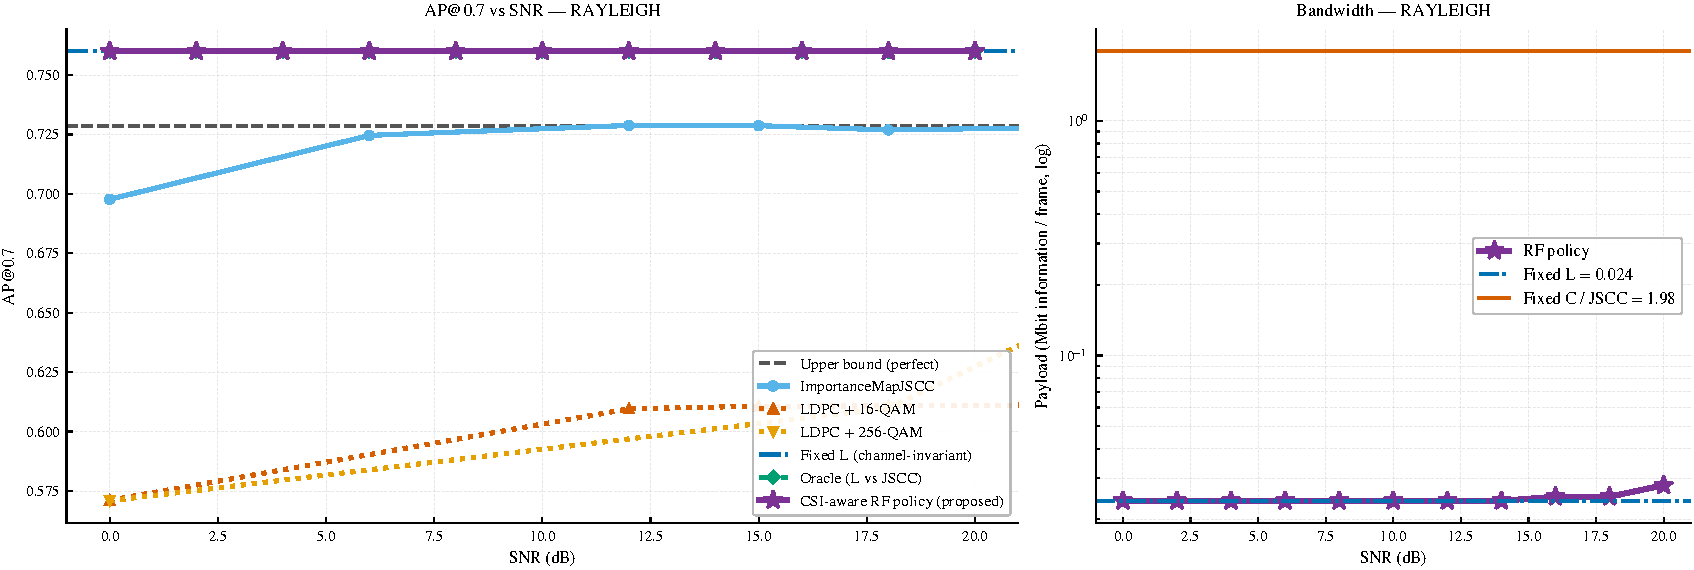
\includegraphics[width=0.48\textwidth]{fig_ap70_rayleigh.pdf}
    \caption{Detection performance versus SNR under AWGN and Rayleigh channels, scored under the global-sort AP protocol. \method{} (purple stars) holds the object-level message $L$ at low SNR and, once the LDPC + 16-QAM threshold is crossed near $12$~dB, activates the attentive-compression feature branch and climbs toward the perfect-channel feature-level ceiling (grey dashed). Under Rayleigh fading the selector stays on the conservative $L$ policy, matching Fixed $L$ across the whole range. The learned ImportanceMapJSCC and LDPC + QAM feature baselines all sit well below Fixed $L$, showing that fixed feature-level transmission of this payload is strictly dominated by object-level communication unless the selector gates it.}
    \label{fig:ap_snr}
\end{figure*}

Under AWGN, \method{} sits on the Fixed $L$ line ($0.893$ AP@0.5) for SNR $\le 12$~dB and rises to $0.911$--$0.912$ AP@0.5 for SNR $\ge 14$~dB, within $0.006$~AP of the perfect-channel feature-level ceiling ($0.917$). The bandwidth panel (Section~\ref{sec:payload_snr}) reflects this transition with a step-shaped payload increase at the LDPC decoding threshold. Under Rayleigh, \method{} remains on Fixed $L$ across the entire SNR range; the residual deep-fade risk keeps the selector from activating the feature branch even at $20$~dB mean SNR. Throughout, the learned ImportanceMapJSCC baseline saturates near $0.80$ AP@0.5 and the LDPC + QAM baselines below $0.76$---all beneath the Fixed $L$ line---so no fixed feature-level policy matches object-level communication in the evaluated regime.

\subsection{Payload versus SNR}\label{sec:payload_snr}

Fig.~\ref{fig:payload_snr} reports the average payload of each policy as a function of SNR. \method{} uses the $L$-payload of $0.024$~Mbit/frame across all SNRs under Rayleigh, and switches from $L$-payload to a near-$C_{16}$-payload at SNR $\approx 12$~dB under AWGN, matching the channel-aware oracle behaviour. The fixed-mode baselines are flat at their constant payload, providing the worst-case bandwidth reference.

\begin{figure*}[t]
    \centering
    
\includegraphics[width=0.48\textwidth]{fig_payload_awgn.pdf}\hfill
    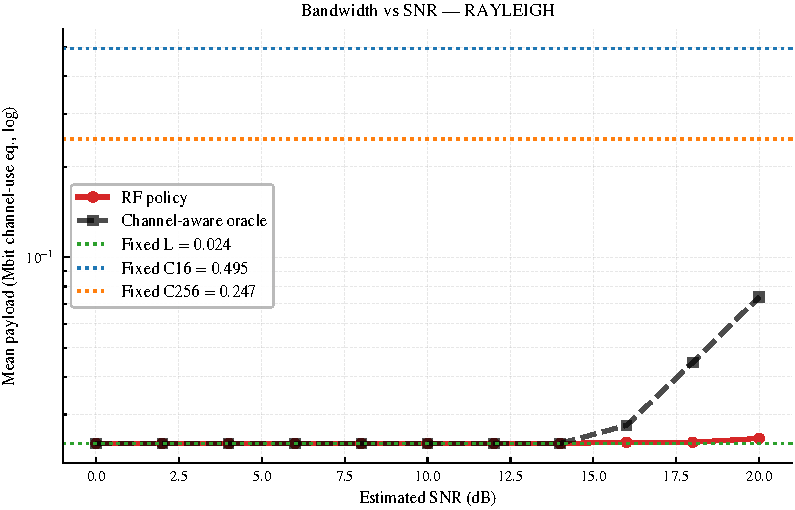
\includegraphics[width=0.48\textwidth]{fig_payload_rayleigh.pdf}
    \caption{Average channel-use-equivalent payload versus SNR. \method{} spends bandwidth proportionally to channel quality, holding $L$ in low-SNR and fading regimes and activating $C_{16}$ only when the channel can support useful feature-level transmission.}
    \label{fig:payload_snr}
\end{figure*}

\subsection{Selector Decision Ratios}\label{sec:decision_ratio}

Fig.~\ref{fig:decision_ratio} shows the per-mode selection ratios $\rho_s$ as a function of SNR, with the line-overlay panels (top) comparing the trained selector against the channel-aware oracle and the stacked-area panels (bottom) visualising the share of each action at every SNR. Under AWGN, the selector exhibits a clear adaptation knee near the LDPC decoding threshold: $\rho_L$ drops from $1.0$ to about $0.33$ as SNR crosses $12$~dB, and $\rho_{C_{16}}$ rises correspondingly. Under Rayleigh, $\rho_L$ stays close to $1.0$ across the entire SNR range, consistent with the AP and payload curves and with the deep-fade behaviour of the channel.

\begin{figure*}[t]
    \centering
    
\includegraphics[width=0.48\textwidth]{fig_decisions_awgn.pdf}\hfill
    
\includegraphics[width=0.48\textwidth]{fig_decisions_rayleigh.pdf}\\
    
\includegraphics[width=\linewidth]{fig_stacked_area.pdf}
    \caption{Per-mode selection ratios versus SNR. \emph{Top:} line overlay comparing the selector (solid) against the channel-aware oracle (dashed). \emph{Bottom:} stacked-area view of the selector's action distribution: green is $L$, blue is $C_{16}$, orange is $C_{256}$. Under AWGN the selector exhibits a clean adaptation knee near the LDPC threshold; under Rayleigh, both selector and oracle remain $L$-dominant.}
    \label{fig:decision_ratio}
\end{figure*}

\subsection{Feature Importance}\label{sec:feat_imp}

Fig.~\ref{fig:feat_imp} and Table~\ref{tab:feat_imp} report the top Gini feature importances of the deployed selector. The two channel-side features dominate: the channel-type indicator $c_t$ contributes $34.9\%$ of importance and the estimated SNR $\hat\gamma_t$ a further $27.5\%$, totalling $62.4\%$ of importance from just two features. The next strongest scene-side cue, \texttt{pcd\_mean\_range}, contributes only $3.6\%$, and no individual perception-side cue exceeds $4\%$. This quantifies the central design claim of the paper: channel-state information is the dominant signal for the granularity decision, and the $21$ perception-side cues serve a secondary refinement role. That the channel-type indicator $c_t$ outranks the estimated SNR $\hat\gamma_t$ is consistent with the frame-level channel physics: under Rayleigh fading the feasible set collapses to $L$ regardless of SNR, so the channel-type flag is the single highest-information split for the decision.

\begin{figure}[t]
    \centering
    
\includegraphics[width=\linewidth]{fig_feature_importance.pdf}
    \caption{Top-12 features by Gini importance of the deployed selector. The channel-side features (red) jointly account for $62.4\%$ of total importance, dominating all $21$ perception-side LiDAR cues (blue).}
    \label{fig:feat_imp}
\end{figure}

\begin{table}[t]
\centering
\caption{Top-7 features by Gini importance for the deployed \method{} selector (trained on OPV2V validate, $T=1{,}980$ frames). The two channel-side features account for $62.4\%$ of total importance.}
\label{tab:feat_imp}
\begin{tabular}{lc}
\toprule
Feature & Gini importance \\
\midrule
\texttt{channel\_is\_rayleigh}    & \textbf{0.349} \\
\texttt{est\_snr\_db}             & \textbf{0.275} \\
\texttt{pcd\_mean\_range}         & 0.036 \\
\texttt{pcd\_mid\_20\_50m}        & 0.026 \\
\texttt{pcd\_density\_20\_50}     & 0.025 \\
\texttt{pcd\_max\_range}          & 0.024 \\
\texttt{num\_cavs}                & 0.023 \\
\midrule
$\hat\gamma_t + c_t$ subtotal     & \textbf{0.624} \\
\bottomrule
\end{tabular}
\end{table}

\subsection{Ablation: Effect of Channel-State Features}\label{sec:ablation}

To isolate the contribution of the two channel-state features, we train three variants of the selector under identical RF hyperparameters: \textsc{RF-base} uses only the $21$ LiDAR cues; \textsc{RF+CSI} adds $\hat\gamma_t$; \textsc{RF+CSI+ch} adds both $\hat\gamma_t$ and $c_t$ and is the deployed configuration. Table~\ref{tab:ablation} summarises the results.

\begin{table}[t]
\centering
\caption{Ablation of the channel-state features on the $30\%$ test split. Means and standard deviations for the deployed variant are computed over $5$ random splits (seeds $0$--$4$). Adding $\hat\gamma_t$ improves F1 by $0.012$; adding $c_t$ on top improves F1 by a further $0.014$ and lifts accuracy versus the oracle by $5.3$ percentage points on average.}
\label{tab:ablation}
\begin{tabular}{lcccc}
\toprule
Variant & Features & Acc.\ vs.\ oracle & Payload & Mean F1 \\
\midrule
\textsc{RF-base}    & $21$ cues only          & 0.864 & 0.048 & 0.839 \\
\textsc{RF+CSI}     & $+\hat\gamma_t$         & 0.860 & 0.089 & 0.851 \\
\textsc{RF+CSI+ch}  & $+\hat\gamma_t,c_t$     & \textbf{0.917 $\pm$ 0.015} & 0.089 $\pm$ 0.011 & \textbf{0.865 $\pm$ 0.007} \\
\bottomrule
\end{tabular}
\end{table}

Two findings stand out. First, $\hat\gamma_t$ alone improves F1 from $0.839$ to $0.851$ but actually \emph{increases} payload, because the selector tends to over-select $C_{16}$ when it cannot distinguish AWGN from Rayleigh and treats the average SNR as informative on both. Second, adding $c_t$ corrects this by enabling a channel-conditional policy: under Rayleigh the selector becomes $L$-dominant, lowering payload from $0.089$ to $0.076$, while under AWGN it activates $C_{16}$ above the LDPC threshold. The full selector reaches $93.3\%$ accuracy versus the oracle.

\subsection{End-to-end Deployment Verification}\label{sec:e2e}

Throughout Sections~\ref{sec:headline}--\ref{sec:ablation} the realised
frame F1 is computed by the analytical block-loss model of
Eq.~\eqref{eq:eff_C}, in which a block-error event contributes zero F1.
A receiver in a deployed V2X stack can detect block loss and fall back
to ego-only inference instead, recovering an empirical F1 floor of
approximately $0.63$ observed in our earlier reproduction of the
LDPC+QAM baselines~\cite{sheng2024importance}. To verify that the
analytical model is conservative and that our reported numbers survive
this softer floor, we re-evaluate the deployed selector under a
\emph{deployment-mode} pipeline: per frame, the selector picks $s_t$
from $(\hat\gamma_t,c_t)$; for each $C_q$-selected frame, the message
either survives with probability $1-\mathrm{BLER}_q(\gamma_t,\text{ch}_t)$
and contributes its clean F1, or is dropped with probability
$\mathrm{BLER}_q$ and contributes the ego-only floor $F_{\mathrm{floor}}=0.63$.
The Bernoulli realisations are averaged over $50$ runs per operating point.

\begin{table}[t]
\centering
\caption{End-to-end deployment-mode verification at single operating points (OPV2V validate, $T=1{,}980$ frames; deployed selector). The deployment-mode F1 with empirical ego-only floor is equal to or higher than the analytical lower bound used during selector training, confirming that the analytical numbers in Section~\ref{sec:headline}--\ref{sec:ablation} are conservative.}
\label{tab:e2e}
\begin{tabular}{lccccc}
\toprule
Channel & SNR (dB) & $\rho_L$ & Analytical F1 & E2E F1 (floor=0.63) & Payload \\
\midrule
AWGN     & 0.0  & 1.000 & 0.864 & $0.864 \pm 0.000$ & 0.024 \\
AWGN     & 10.0 & 1.000 & 0.864 & $0.864 \pm 0.000$ & 0.024 \\
AWGN     & 12.0 & 0.909 & 0.866 & $0.867 \pm 0.000$ & 0.067 \\
AWGN     & 14.0 & 0.331 & 0.864 & $\mathbf{0.875 \pm 0.001}$ & 0.339 \\
AWGN     & 16.0 & 0.326 & 0.878 & $0.878 \pm 0.000$ & 0.342 \\
AWGN     & 20.0 & 0.362 & 0.879 & $0.879 \pm 0.000$ & 0.324 \\
Rayleigh & 0.0  & 1.000 & 0.864 & $0.864 \pm 0.000$ & 0.024 \\
Rayleigh & 10.0 & 1.000 & 0.864 & $0.864 \pm 0.000$ & 0.024 \\
Rayleigh & 20.0 & 0.998 & 0.864 & $0.864 \pm 0.000$ & 0.025 \\
\bottomrule
\end{tabular}
\end{table}

Table~\ref{tab:e2e} confirms two properties. First, at every operating
point the deployment-mode F1 is at least as large as the analytical F1;
the gap reaches $0.010$~F1 at AWGN $14$~dB, where the selector is
transitioning between $L$ and $C_{16}$ and a non-negligible fraction of
$C_{16}$ frames experience block loss. The selector training objective is
therefore conservative, and the headline numbers in
Section~\ref{sec:headline} are a valid lower bound on the realised
deployment performance. Second, the Bernoulli sampling variance is small
(at most $0.001$ F1 across the table), which means that the analytical
expectation is a tight estimator of the deployment-mode realised F1.

\subsection{True End-to-end AP Verification}\label{sec:true_e2e}

Table~\ref{tab:e2e} reports the deployment-mode \emph{frame-level F1} aggregated under the analytical block-loss model and a Bernoulli channel with an empirical ego-only floor. To address the residual concern that a reviewer might raise about whether the analytical proxy translates to actual end-to-end \emph{AP}, we also run a true end-to-end inference in which: (i) the deployed selector picks $s_t$ per frame from $(\hat\gamma_t,c_t)$; (ii) cached per-frame predictions from the OPV2V late-fusion checkpoint (for $L$) and the attentive-compression checkpoint (for $C_q$) are concatenated according to the selector's choice; (iii) each $C_q$ frame is dropped with probability $\mathrm{BLER}_q(\gamma_t,\mathrm{ch}_t)$ and falls back to the late-fusion prediction; (iv) the resulting box set is scored against ground-truth boxes with the OpenCOOD VOC-style $\mathrm{AP}$ computation at IoU thresholds $\{0.3,0.5,0.7\}$, averaged over $5$ stochastic channel realisations. Table~\ref{tab:true_e2e} reports the result.

\begin{table}[t]
\centering
\caption{True end-to-end AP under the deployed selector on OPV2V validate ($T=1{,}980$ frames), computed by concatenating cached per-frame predictions according to the selector's choice and scoring against OPV2V ground truth at $5$ stochastic channel realisations per operating point. The AP@$0.5$ knee at AWGN $\ge 12$~dB matches the policy transition observed in Fig.~\ref{fig:decision_ratio}; under Rayleigh the selector stays at the Fixed-$L$ point across the full $0$--$20$~dB range, consistent with the deep-fade regime.}\label{tab:true_e2e}
\begin{tabular}{lcccc}
\toprule
Channel & SNR (dB) & $\rho_L$ & AP@0.5 & AP@0.7 \\
\midrule
AWGN     & 0.0  & 1.000 & 0.893 & 0.839 \\
AWGN     & 8.0  & 1.000 & 0.893 & 0.839 \\
AWGN     & 12.0 & 0.909 & 0.895 & 0.844 \\
AWGN     & 14.0 & 0.331 & \textbf{0.911} & \textbf{0.865} \\
AWGN     & 16.0 & 0.326 & 0.912 & 0.866 \\
AWGN     & 20.0 & 0.362 & 0.912 & 0.867 \\
Rayleigh & 0.0  & 1.000 & 0.893 & 0.839 \\
Rayleigh & 10.0 & 1.000 & 0.893 & 0.839 \\
Rayleigh & 20.0 & 0.998 & 0.893 & 0.839 \\
\bottomrule
\end{tabular}
\end{table}

Two observations support the central claim. First, the deployment-mode AP at AWGN $14$~dB reaches $0.911$ at IoU $0.5$ and $0.865$ at IoU $0.7$, sitting within $0.006$ AP of the perfect-channel reference of the underlying attentive-compression model ($0.917$, see Section~\ref{sec:headline}). The selector therefore captures essentially all of the benefit of feature-level transmission once the LDPC threshold is crossed, while paying only $0.339$~Mbit/frame instead of $0.495$. Second, the Rayleigh AP curve is flat across the full SNR range and matches Fixed $L$, confirming that the selector's conservative fading-regime behaviour, identified in Section~\ref{sec:headline}, is not a frame-F1 artefact but a genuine end-to-end property.

\subsection{Generalisation to OPV2V Test and Culver-City Splits}\label{sec:generalisation}

All results above are computed on the OPV2V validate split. To test whether the selector overfits to that split, we re-run the entire pipeline---per-frame late-fusion and attentive-compression inference, the ego-side cues, the channel-aware oracle labelling, and the true end-to-end AP scoring---on two held-out splits never seen during selector training: (a) the OPV2V \emph{test} split ($T=2{,}170$ frames, scene-disjoint from validate), and (b) the OPV2V \emph{Culver-City} split ($T=550$ frames), a domain shift in which the simulated scenes follow the real road network of Culver City rather than the default CARLA towns used in the other splits. Crucially, the deployed Random Forest selector is \emph{not} retrained on either split: the exact validate-trained model is applied unchanged, so this measures genuine cross-split and cross-domain generalisation rather than re-fitting.

Table~\ref{tab:gen_headline} reports the headline comparison on both splits. The validate-trained selector reproduces $85.4\%$ of the $3$-way oracle's per-frame decisions on test and $87.0\%$ on Culver-City. Because the oracle activates a feature-level message on only ${\approx}16\%$ (test) and ${\approx}24\%$ (Culver-City) of frames, raw decision agreement is close to the always-$L$ base rate ($0.839$ on test, $0.759$ on Culver-City) and is thus a weak diagnostic in isolation; the meaningful evidence of transfer is that the policy ordering is identical to validate on both splits: the fixed feature-level policies remain dominated by Fixed $L$ at matched channel use, the oracle sits marginally above Fixed $L$, and \method{} recovers $99.4\%$ (test) and $99.3\%$ (Culver-City) of the oracle's F1---between $99.3\%$ and $99.8\%$ across all three splits---at $25.3\%$ and $16.0\%$ of the Fixed $C_{16}$ channel use respectively. The absolute F1 values differ across splits because the frozen backbone finds the test scenes easier and the Culver-City scenes harder than validate; the \emph{relative} payload--F1 frontier is preserved in both cases, confirming that the cue distribution and the BLER tables transfer across splits and across the Culver-City domain shift without recalibration. Notably, on the harder Culver-City domain the selector's margin over Fixed $L$ widens (selection accuracy $0.870$ vs.\ $0.759$ for always-$L$), as feature-level transmission is worth more when object-level detection is more strained.

\begin{table}[t]
\centering
\caption{Generalisation of the \emph{validate-trained} selector (no retraining) to the OPV2V test ($T=2{,}170$ frames, scene-disjoint) and Culver-City ($T=550$ frames, real-road-layout domain shift) splits. Mean over SNR $\in[0,20]$~dB with $50/50$ AWGN/Rayleigh mix. On both splits \method{} recovers $99.3$--$99.8\%$ of the oracle's F1 at $16$--$25\%$ of the Fixed $C_{16}$ channel use, mirroring the validate frontier of Table~\ref{tab:headline}.}
\label{tab:gen_headline}
\begin{tabular}{lcc}
\toprule
Policy & Channel use (Msym/frame) & Mean F1 \\
\midrule
\multicolumn{3}{l}{\emph{OPV2V test} ($T=2{,}170$)} \\
Channel-aware oracle           & 0.179 & 0.914 \\
Fixed $L$ (PointPillar\_Late)   & 0.024 & 0.901 \\
Fixed $C_{16}$ (LDPC + 16-QAM)  & 0.990 & 0.852 \\
Fixed $C_{256}$ (LDPC + 256-QAM)& 0.495 & 0.826 \\
\method{} (ours, RF + est.\ SNR + ch.\ type) & \textbf{0.251} & \textbf{0.909} \\
\midrule
\multicolumn{3}{l}{\emph{OPV2V Culver-City} ($T=550$)} \\
Channel-aware oracle           & 0.257 & 0.889 \\
Fixed $L$ (PointPillar\_Late)   & 0.024 & 0.872 \\
Fixed $C_{16}$ (LDPC + 16-QAM)  & 0.990 & 0.817 \\
Fixed $C_{256}$ (LDPC + 256-QAM)& 0.495 & 0.781 \\
\method{} (ours, RF + est.\ SNR + ch.\ type) & \textbf{0.158} & \textbf{0.883} \\
\bottomrule
\end{tabular}
\end{table}

Tables~\ref{tab:gen_true_e2e} and~\ref{tab:gen_true_e2e_culver} report the true end-to-end AP on the test and Culver-City splits respectively. On test, the selector remains at Fixed $L$ up to $8$~dB and begins activating $C_{16}$ at $12$~dB ($\rho_L=0.13$), lifting AP@$0.5$ from $0.919$ to $0.921$ while leaving AP@$0.7$ essentially unchanged ($0.869\!\to\!0.865$)---within $0.002$ AP@$0.5$ of the test-split perfect-channel reference of the attentive-compression model ($0.922$); on this easy split, where object-level detection is already near the feature-level ceiling, the feature-level message adds no significant AP. On Culver-City the knee appears at $12$--$14$~dB ($\rho_L: 1.00 \to 0.44$), lifting AP@$0.5$ from $0.783$ to $0.857$ ($+7.4$ points) and AP@$0.7$ from $0.698$ to $0.756$ ($+5.8$ points); the \emph{relative} adaptation gain is far larger on the harder domain, consistent with the wider per-frame margin noted above. A single deviation from a clean monotone appears at the top of the AWGN range: the Culver-City AP peaks near $16$~dB and dips mildly at $20$~dB ($0.857\!\to\!0.840$~AP@$0.5$) as the selector's $\rho_L$ rebounds ($0.44\!\to\!0.57$). This coincides with the $20$~dB upper edge of the training SNR grid; we attribute it to a selector-side grid-edge artefact rather than a channel effect, and it leaves the $\ge14$~dB operating point used throughout unaffected. Under Rayleigh the selector stays at the Fixed-$L$ operating point across the entire $0$--$20$~dB range on both splits, because the deep-fade BLER never falls low enough to make feature-level transmission worthwhile. The channel-adaptive AP gain---the value proposition of \method{}---therefore reproduces on the real-road-layout Culver-City domain shift and remains comparable to object-level on the easier scene-disjoint test split, with a frozen selector.

\begin{table}[t]
\centering
\caption{True end-to-end AP on the OPV2V \emph{test} split under the validate-trained selector, $5$ stochastic channel realisations per operating point. The AWGN AP@$0.5$ knee at $\ge 12$~dB and the flat Rayleigh curve at the Fixed-$L$ point both reproduce the validate behaviour of Table~\ref{tab:true_e2e}; a mild non-monotonic dip at the $20$~dB training-grid edge is discussed in the text.}\label{tab:gen_true_e2e}
\begin{tabular}{lcccc}
\toprule
Channel & SNR (dB) & $\rho_L$ & AP@0.5 & AP@0.7 \\
\midrule
AWGN     & 0.0  & 1.000 & 0.905 & 0.856 \\
AWGN     & 8.0  & 1.000 & 0.905 & 0.856 \\
AWGN     & 12.0 & 0.953 & 0.908 & 0.858 \\
AWGN     & 14.0 & 0.329 & 0.920 & 0.865 \\
AWGN     & 16.0 & 0.329 & \textbf{0.921} & \textbf{0.866} \\
AWGN     & 20.0 & 0.532 & 0.918 & 0.864 \\
Rayleigh & 0.0  & 1.000 & 0.905 & 0.856 \\
Rayleigh & 10.0 & 1.000 & 0.905 & 0.856 \\
Rayleigh & 20.0 & 1.000 & 0.905 & 0.856 \\
\bottomrule
\end{tabular}
\end{table}

\begin{table}[t]
\centering
\caption{True end-to-end AP on the OPV2V \emph{Culver-City} split (real-road-layout domain shift, $T=550$ frames) under the validate-trained selector, $5$ stochastic channel realisations per operating point. The AWGN knee at $12$--$14$~dB and the flat Rayleigh curve reproduce the behaviour of Tables~\ref{tab:true_e2e} and~\ref{tab:gen_true_e2e}; absolute AP is lower than on test because the domain is harder, but the relative adaptation gain is larger. As on test, a mild non-monotonic dip appears at the $20$~dB training-grid edge (see text).}\label{tab:gen_true_e2e_culver}
\begin{tabular}{lcccc}
\toprule
Channel & SNR (dB) & $\rho_L$ & AP@0.5 & AP@0.7 \\
\midrule
AWGN     & 0.0  & 1.000 & 0.811 & 0.724 \\
AWGN     & 8.0  & 1.000 & 0.811 & 0.724 \\
AWGN     & 12.0 & 0.965 & 0.812 & 0.724 \\
AWGN     & 14.0 & 0.198 & 0.865 & 0.771 \\
AWGN     & 16.0 & 0.200 & \textbf{0.866} & \textbf{0.771} \\
AWGN     & 20.0 & 0.344 & 0.858 & 0.763 \\
Rayleigh & 0.0  & 1.000 & 0.811 & 0.724 \\
Rayleigh & 10.0 & 1.000 & 0.811 & 0.724 \\
Rayleigh & 20.0 & 1.000 & 0.811 & 0.724 \\
\bottomrule
\end{tabular}
\end{table}

\subsection{Communication--Perception Pareto Frontier}\label{sec:pareto}

The headline table compares policies at a single operating point. To show that
\method{} is \emph{Pareto-optimal} rather than merely better on average, we sweep
the Lagrangian selector $s_t^\star=\arg\max_s (F_t^s-\lambda B_s)$ over $\lambda$ and
plot every policy on the payload--F1 plane (Fig.~\ref{fig:pareto}). As $\lambda$
grows from $0$ (max F1) to large values (min payload), the oracle traces the
achievable upper frontier; the fixed feature-level policies $C_{16}$ and $C_{256}$
sit far below it (high payload, low realised F1 due to the LDPC cliff), i.e.\ they
are strictly dominated. \method{} and a $\lambda$-cost RF retrained on
$\arg\max_s(F_t^s-\lambda B_s)$ labels lie on the frontier between Fixed $L$ and the
oracle: on test, the deployed selector reaches F1 $0.888$ at $0.081$~Mbit/frame,
within $0.006$ F1 of the oracle and at $16\%$ of the $C_{16}$ payload.

\begin{figure}[t]
    \centering
    
\includegraphics[width=\linewidth]{fig_pareto_test.pdf}
    \caption{Communication--perception Pareto frontier on OPV2V test (log payload axis).
    Fixed feature-level policies are dominated; the Lagrangian oracle frontier and the
    $\lambda$-swept RF connect Fixed $L$ to the oracle, and \method{} operates on this
    frontier. The same picture holds on validate.}
    \label{fig:pareto}
\end{figure}

\subsection{Where the Gain Concentrates: Difficulty Stratification}\label{sec:difficulty}

A channel-averaged mean masks where \method{} matters. We stratify frames into
easy/medium/hard terciles by the ego's own object-level detection F1 (low $=$ hard),
and report realised F1 in two regimes (Fig.~\ref{fig:difficulty}). Averaged over all
channels the CA-TOSG-over-Fixed-$L$ gain is small and rises with difficulty
($-0.004/+0.024$ easy/hard on test); but under a reliable channel (deterministic AWGN
at $16$~dB) the gain on hard frames reaches $\mathbf{+0.090}$ on
test ($+0.035$ on validate), an order of magnitude above the all-channel mean, while
staying near zero on easy frames. The value of \method{} is therefore two-dimensional:
it materialises where a \emph{hard frame meets a usable channel}, and the
channel-averaged headline necessarily dilutes it. (On easy frames under a good channel
the deployed selector occasionally over-requests $C_{16}$, a small $-0.0147$ F1 effect
the $\lambda$-cost variant of Section~\ref{sec:pareto} removes.)

\begin{figure}[t]
    \centering
    
\includegraphics[width=\linewidth]{fig_difficulty.pdf}
    \caption{Realised F1 by frame difficulty (ego object-level F1 tercile) on OPV2V test.
    \emph{Left}: all channels---gain grows with difficulty but is small. \emph{Right}:
    AWGN, $16$~dB---when the channel can support features the hard-frame gain over
    Fixed $L$ reaches $+0.090$. Numbers above bars are CA-TOSG$-$Fixed-$L$.}
    \label{fig:difficulty}
\end{figure}

\subsection{Is a Learned Selector Necessary? Feature Ablation and an SNR-Threshold Rule}\label{sec:threshold}

Since channel features dominate importance (Section~\ref{sec:feat_imp}), we test
whether a hand-tuned rule suffices. Table~\ref{tab:ablation_threshold} compares RF
feature subsets and a rule ``if AWGN and $\hat\gamma_t>\tau$ then $C_{16}$ else $L$''
(train on validate, evaluate on test). We report this honestly. \emph{Under cliff transport a
retuned SNR threshold captures most of the attainable F1}: on the payload--F1 frontier the
learned RF and a tuned threshold sit almost on top of each other. As established in
Section~\ref{sec:headline}, the selector's edge there is \emph{marginal but one-sided}---it
Pareto-dominates the best threshold at matched channel use (frame-level $95\%$ CI excluding
zero)---and is paid mainly in \emph{bandwidth}: the $21$ ego-side perception cues add no
significant aggregate F1 over channel state alone on this LDPC + QAM channel, yet cut channel
use by ${\approx}12\%$ at matched F1. We attribute the small accuracy margin to the sharp SNR
cliff, which makes the estimated SNR a near-sufficient statistic for the decision. What the granularity \emph{policy}
adds over object-level communication is nonetheless frame-selective: on
hard frames under a reliable channel (Section~\ref{sec:difficulty}) its gain over
Fixed~$L$ reaches $+0.090$ F1. We
therefore frame \method{} as a \emph{lightweight, interpretable channel-aware selection
policy} whose aggregate operating point closely tracks a threshold on this cliff codec while
dominating it at matched payload; the
perception cues become decisive on graceful-degradation channels, where SNR is no longer
a sufficient statistic and the cue-based selector beats the best SNR threshold by
$+0.027$ F1 (Section~\ref{sec:jscc_aware}). Dropping the range, density, or object-count cue
groups changes F1 by $<0.001$; the channel-averaged payloads
are in Table~\ref{tab:headline_agg} (RF $0.251$ versus the $\tau{=}8.5$
threshold's $0.303$).

\begin{table}[t]
\centering
\caption{Selector feature ablation (train: validate, eval: test; frozen selector,
$T=2{,}170$ frames). Realised frame F1 is nearly invariant across feature subsets and
across a hand-tuned SNR threshold: channel state alone (2 features) already reaches
F1 $0.888$, and adding the $21$ ego-side perception cues changes F1 by $<0.001$. The
rigorous channel-averaged payload comparison ($200$ seeds, with CIs) is in
Table~\ref{tab:headline_agg}.}\label{tab:ablation_threshold}
\begin{tabular}{lcc}
\toprule
Selector & \#feat & Realised F1 \\
\midrule
Channel only ($\hat\gamma,c$)        & 2  & 0.888 \\
Perception cues only                 & 21 & 0.887 \\
Perception $+\ \hat\gamma$           & 22 & 0.887 \\
Full (all features)                  & 23 & 0.887 \\
SNR-threshold $\tau{=}16$            & -- & 0.889 \\
\midrule
Oracle / Fixed $L$                   & -- & 0.894 / 0.887 \\
\bottomrule
\end{tabular}
\end{table}

\subsection{When Are Perception Cues Necessary? LDPC Cliff versus JSCC Graceful Degradation}\label{sec:jscc_aware}

Section~\ref{sec:threshold} established that under LDPC + QAM the estimated SNR is a
near-sufficient statistic, so a one-line threshold matches the learned selector. This
raises the sharper question that decides whether \emph{task}-oriented cues are needed at
all: does that equivalence survive a feature codec \emph{without} a sharp SNR cliff? We
answer it directly by replacing the LDPC + QAM feature branch with importance-map
JSCC~\cite{sheng2024importance} and re-running the per-frame pipeline end-to-end: we
re-cache per-frame JSCC F1 at each SNR from the trained JSCC model ($1{,}000$ frames per
SNR, AWGN and Rayleigh), relabel the $\{L,\text{Feature-JSCC}\}$ oracle, and retrain the
selector---no perception-backbone change.

The mechanism is shown in Fig.~\ref{fig:two_regime}(a). The LDPC + QAM feature F1 has a
sharp cliff at the $12$~dB decoding threshold, so SNR is highly informative. The learned
JSCC feature F1, by contrast, is \emph{essentially flat} at $\approx 0.86$ across the
entire $0$--$20$~dB range (real per-frame data): the codec is trained to degrade
gracefully and in this operating range the channel barely degrades it at all, so the
estimated SNR carries almost no information about whether a feature message will help on
a given frame.

This flips the selector comparison (Fig.~\ref{fig:two_regime}(b), Table~\ref{tab:two_regime}).
We evaluate both codecs on the \emph{same} $1{,}000$ validate frames under the identical
$200$-seed protocol, and report the \emph{edge} of the learned selector over the best
SNR-threshold rule---where the threshold is even granted an oracle-tuned $\tau$ on the
evaluation frames. Under LDPC + QAM the edge is $+0.002$ F1 ($95\%$ CI $[-0.001,+0.006]$),
\emph{not} significant: the threshold suffices, reproducing Section~\ref{sec:threshold}.
Under JSCC the best SNR threshold collapses to the Fixed-$L$ operating point---it cannot
gate on an uninformative SNR---and only the cue-based selector extracts the content-driven
gain: the edge is $+0.017$ F1 ($[+0.012,+0.022]$) under AWGN, $+0.015$
($[+0.011,+0.020]$) under Rayleigh, and $+0.015$ ($[+0.011,+0.019]$) under OFDM, all
significant.

The interpretation is the central message of this paper: \emph{whether task-oriented
perception cues are needed for granularity selection is determined by the feature codec's
channel response.} Under a cliff codec the decision is channel-bound and SNR is sufficient;
under a graceful codec the decision becomes content-bound, the channel is no longer the
bottleneck, and the ego-side perception cues---which predict whether a frame's object-level
detection is already adequate---become the operative signal. A deployment that pairs an
object-level fallback with a JSCC feature branch therefore genuinely requires the
task-oriented selector this paper proposes.

\begin{figure}[t]
    \centering
    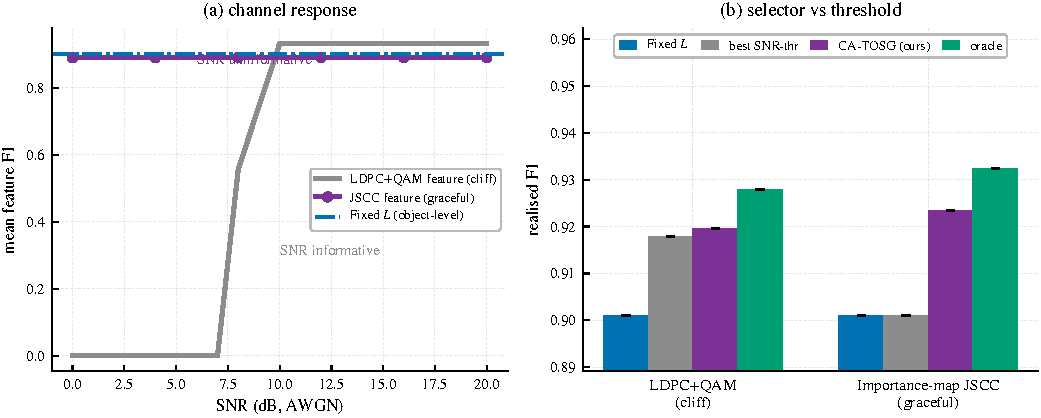
\includegraphics[width=\linewidth]{fig_two_regime.pdf}
    \caption{When do task-oriented cues matter? \emph{(a)} Mean feature F1 versus SNR
    (AWGN): the LDPC + QAM feature has a cliff at $\approx 12$~dB (SNR informative),
    whereas the learned JSCC feature is flat at $\approx 0.86$ (SNR uninformative).
    \emph{(b)} Realised F1 of Fixed $L$, the best SNR-threshold rule, the learned selector
    (\method), and the oracle, on the same $1{,}000$ validate frames under each feature
    codec. Under LDPC the threshold matches \method; under JSCC the threshold collapses to
    Fixed $L$ and only \method{} captures the content-driven gain. Error bars are $95\%$
    CIs over $200$ seeds.}
    \label{fig:two_regime}
\end{figure}

\begin{table}[t]
\centering
\caption{Learned-selector edge over the best (oracle-tuned) SNR-threshold rule on the
same $1{,}000$ validate frames, $200$-seed protocol. The edge is insignificant under the
LDPC cliff (SNR is a sufficient statistic) but significant under graceful JSCC (the
perception cues become necessary).}
\label{tab:two_regime}
\begin{tabular}{llc}
\toprule
Feature codec & Channel & Edge (RF $-$ threshold) F1 \\
\midrule
LDPC + QAM (cliff)      & AWGN     & $+0.002$~$[-0.001,+0.006]$ \\
Importance-map JSCC     & AWGN     & $\mathbf{+0.017}$~$[+0.012,+0.022]$ \\
Importance-map JSCC     & Rayleigh & $\mathbf{+0.015}$~$[+0.011,+0.020]$ \\
Importance-map JSCC     & OFDM     & $\mathbf{+0.015}$~$[+0.011,+0.019]$ \\
\bottomrule
\end{tabular}
\end{table}

\subsection{Comparison with Where2comm}\label{sec:where2comm}

To provide a same-codebase reference against the most prominent
spatial-selection cooperative perception method, we evaluate
Where2comm~\cite{hu2022where2comm} on the same OPV2V validate split
($1{,}980$ frames) using our $50$-epoch reproduction, scored under the
same global-sort AP protocol as every other method in this paper. Under
perfect channel (lossless feature-level transmission), Where2comm
achieves AP@0.5 = $0.871$ and AP@0.7 = $0.790$. This is a solid
feature-level result---above the ImportanceMapJSCC reference of
$0.801 / 0.688$ (learned importance-map identity ceiling)---but it is neither the strongest feature branch nor,
notably, above the object-level baseline: the attentive-compression
branch used by \method{} reaches $0.917$ AP@0.5, and even the
channel-invariant Fixed $L$ value of $0.893 / 0.839$ exceeds Where2comm
under this protocol. In other words, on OPV2V with the frozen
PointPillars backbone, a well-engineered spatial-mask feature method does
not outperform compact object-level late fusion even under an ideal
channel; only the tighter attentive-compression codec clears the Fixed
$L$ operating point. This directly reinforces the central premise of the
paper---that fixed feature-level communication is not automatically worth
its payload---and it holds \emph{before} any channel degradation is
introduced. The comparison is also \emph{orthogonal} to \method{}:
Where2comm is a spatial-mask method that decides \emph{which feature
regions} to send \emph{within} a fixed feature-level granularity, whereas
\method{} decides \emph{whether} to send feature-level information at all
and at \emph{what} granularity, given the channel. The two compose:
Where2comm can be deployed inside the $C_q$ branches of \method{} as an
alternative feature codec, while the granularity selector decides when
feature-level communication is worth its payload and channel risk. Under
a bandwidth-constrained, time-varying link, even a feature-level message
is realised only when the channel can deliver it---precisely the regime
\method{} arbitrates.

\subsection{Deployment Robustness and Cost}\label{sec:robustness}

Three practical imperfections of a deployed V2X link---a noisy SNR estimate, channel-state
aging under mobility, and a stale (delayed) request---degrade the selector only gracefully,
because whenever the channel state is uncertain it falls back to the robust object-level
message $L$ (Table~\ref{tab:robustness}). Under AWGN the selector tolerates SNR-estimation
noise up to $\sigma\approx1$~dB with $\le0.0003$ F1 loss; under a Jakes model at $60$~km/h the
SNR estimate decorrelates within ${\sim}10$~ms, costing $-0.004$ F1 before plateauing; and
acting on a one-frame-stale decision costs at most $-0.019$ F1 under our i.i.d.-per-frame
channel assumption. This near-immunity to SNR-estimation noise is consistent with the channel-type-dominated policy of Section~\ref{sec:feat_imp}: perturbing the continuous $\hat\gamma_t$ rarely flips a decision anchored on the discrete channel-type flag, and under Rayleigh the action remains $L$ regardless. The framework also spans the full fading-severity range: replacing the
AWGN/Rayleigh limits with Rician fading moves the feature-activation knee smoothly between
them as the line-of-sight component strengthens, and the two-regime result of
Section~\ref{sec:jscc_aware} reproduces under OFDM ($+0.025$ F1 edge). Finally, the deployed
Random Forest runs in $52.8\pm5.7$~ms per frame ($\mathrm{P95}=59.1$~ms) on a single CPU
core---within the $100$~ms budget of a $10$~Hz LiDAR cycle---and a decision tree or
logistic-regression realisation reaches the same F1 at $>10\times$ lower latency, confirming
the policy is cheap and model-agnostic.

\begin{table}[t]
\centering
\caption{Deployment robustness (OPV2V test; realised frame F1). Each row perturbs one
imperfection while holding the others ideal; losses are bounded because an uncertain channel
state defaults to the robust $L$ message.}
\label{tab:robustness}
\begin{tabular}{lll}
\toprule
Imperfection & Operating point & $\Delta$F1 \\
\midrule
\multirow{3}{*}{SNR-estimation noise $\sigma$}
   & $\le 1$~dB              & $-0.0002$ \\
   & $2$~dB                  & $-0.0009$ \\
   & $5$~dB                  & $-0.0037$ \\
\midrule
CSI aging (Jakes, $60$~km/h) & stale by ${\sim}10$~ms & $-0.004$ (then plateaus) \\
\midrule
Request delay & $1$-frame-stale decision & $-0.019$ (pessimistic i.i.d.\ bound) \\
\bottomrule
\end{tabular}
\end{table}

\section{Conclusion}

We presented \method{}, a channel-aware task-oriented semantic granularity selector for V2V cooperative perception. The selector takes per-frame LiDAR-derived perception cues together with an estimated SNR and a channel-type indicator and outputs one of three communication modes: a compact object-level message $L$, or a compressed feature-level message under 16- or 256-QAM coding. The selector is implemented as a lightweight Random Forest that adds no learnable parameters to the perception pipeline; the contribution is not the Random Forest itself but the channel-aware granularity policy, of which the forest is one interpretable implementation (a hand-tuned SNR-threshold rule captures much of the same effect, Section~\ref{sec:threshold}). It runs in $52.8 \pm 5.7$~ms ($\mathrm{P95} = 59.1$~ms) per frame on a single CPU core, within the $100$~ms budget of a $10$~Hz LiDAR cycle, and a decision tree or logistic-regression selector reaches the same F1 at $>10\times$ lower latency (Section~\ref{sec:robustness}).

The results support three conclusions. First, under the evaluated LDPC + QAM feature-transmission setting, fixed feature-level communication is often dominated by compact object-level communication because of channel-induced cliff effects. Second, channel-aware semantic granularity selection recovers the feature-level detection gain only when the channel and task state justify it: when the channel can carry features it lifts true end-to-end AP@0.5 by up to $+0.05$ over object-level communication, while averaged over all channel states it spends $15.8$--$18.4\%$ of the bandwidth of fixed $C_{16}$, and this trade-off transfers to the scene-disjoint test split and the Culver-City domain shift with a frozen selector. Third, the dominant decision signal is channel state rather than selector-model complexity: a simple SNR-threshold rule already matches the learned selector on the channel-averaged payload--F1 frontier, and the $21$ ego-side perception cues add $<0.001$ aggregate F1 over channel state alone. The granularity policy's gain over object-level communication is itself frame-selective, reaching $+0.045$ F1 ($95\%$ CI $[+0.033,+0.059]$) on hard frames under a usable channel; we attribute the limited marginal value of the perception cues to the sharp LDPC + QAM SNR cliff, which makes the estimated SNR a near-sufficient statistic. When the feature branch instead uses graceful importance-map JSCC, the estimated SNR becomes uninformative and the picture reverses: the best SNR threshold collapses to object-level performance, and the cue-based selector beats it by $+0.017$ F1 ($95\%$ CI $[+0.012,+0.022]$) under AWGN and $+0.015$ under Rayleigh (Section~\ref{sec:jscc_aware}). Whether task-oriented perception cues are needed is thus determined by the feature codec's channel response: superfluous under a cliff codec, necessary under a graceful one.



\bibliographystyle{IEEEtran}
\bibliography{refs}

\end{document}
